\section{Mecanismos de busca e internet}


\begin{frame}{Introdução}
	\begin{block}{}
		\begin{itemize}
			\item Você, com certeza, já se deparou com algo que não sabia, e teve que pesquisar no \textit{Google}, ou perguntar à alguém.
			\item Pode não parecer, mas essa situação corriqueira exige diversos passos, e podemos utilizar estratégias para otimizar a pesquisa na internet.
			\item Nessa aula vamos estudar isso.
		\end{itemize}
	\end{block}

	\bigskip

	\centering
	
\includegraphics[width=0.7\linewidth]{Figuras/Ch03/fig1.1}
\end{frame}


\begin{frame}{Mecanismos de busca}
	\begin{block}{O que são?}
		\begin{itemize}
			\item \textbf{Mecanismos de busca} são ferramentas que, a partir de uma entrada do usuário, exibem conteúdo relacionado.
			\item Por exemplo, pesquisando ``gatos'' no Google, podemos encontrar os seguintes resultados:
		\end{itemize}
	\end{block}

	\centering
	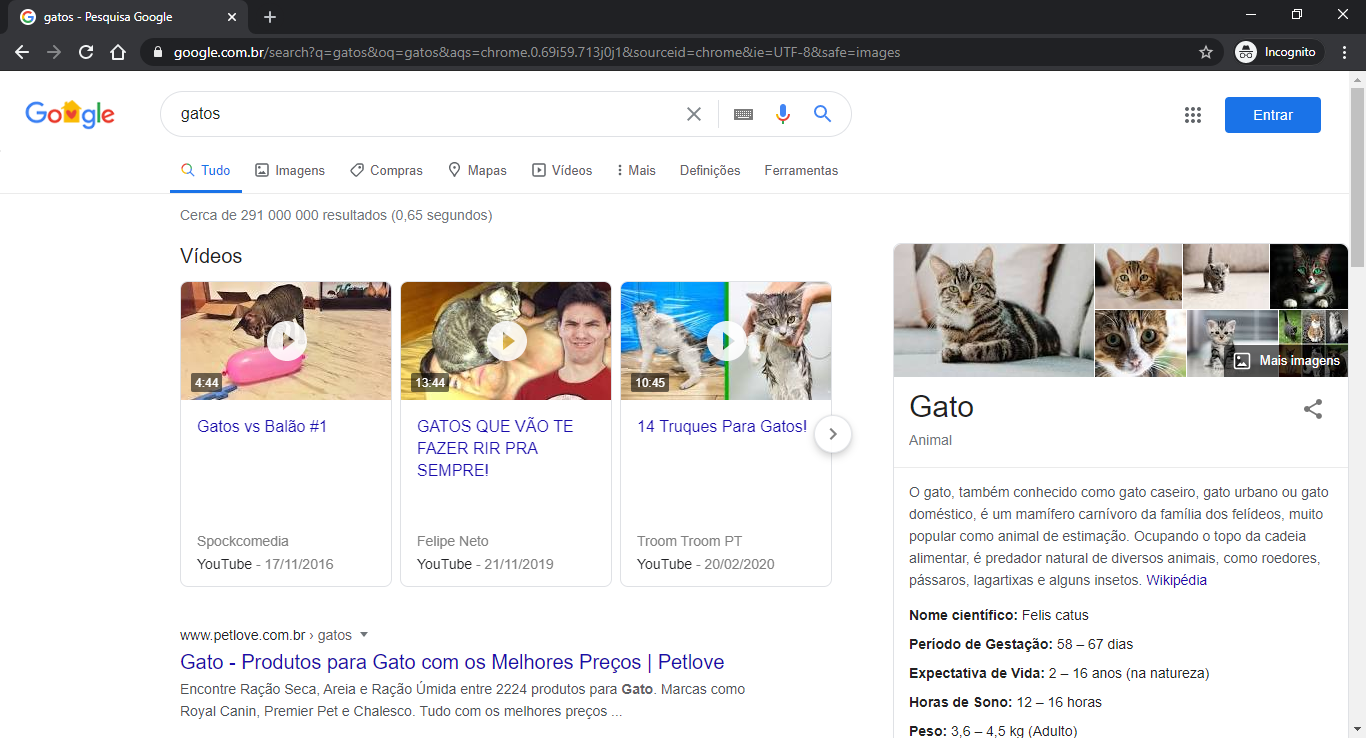
\includegraphics[width=0.75\linewidth]{Figuras/Ch03/fig1}
\end{frame}

\begin{frame}{Mecanismos de busca}
	\begin{block}{}
		\begin{itemize}
			\item Repare que, convenientemente, o Google já organiza uma página com vídeos e fotos de gatos, definições do que seria um gato, além de vários outros links úteis, que ele acha que vão nos agradar, em \textbf{ordem de prioridade}.
		\end{itemize}
	\end{block}

	\centering
	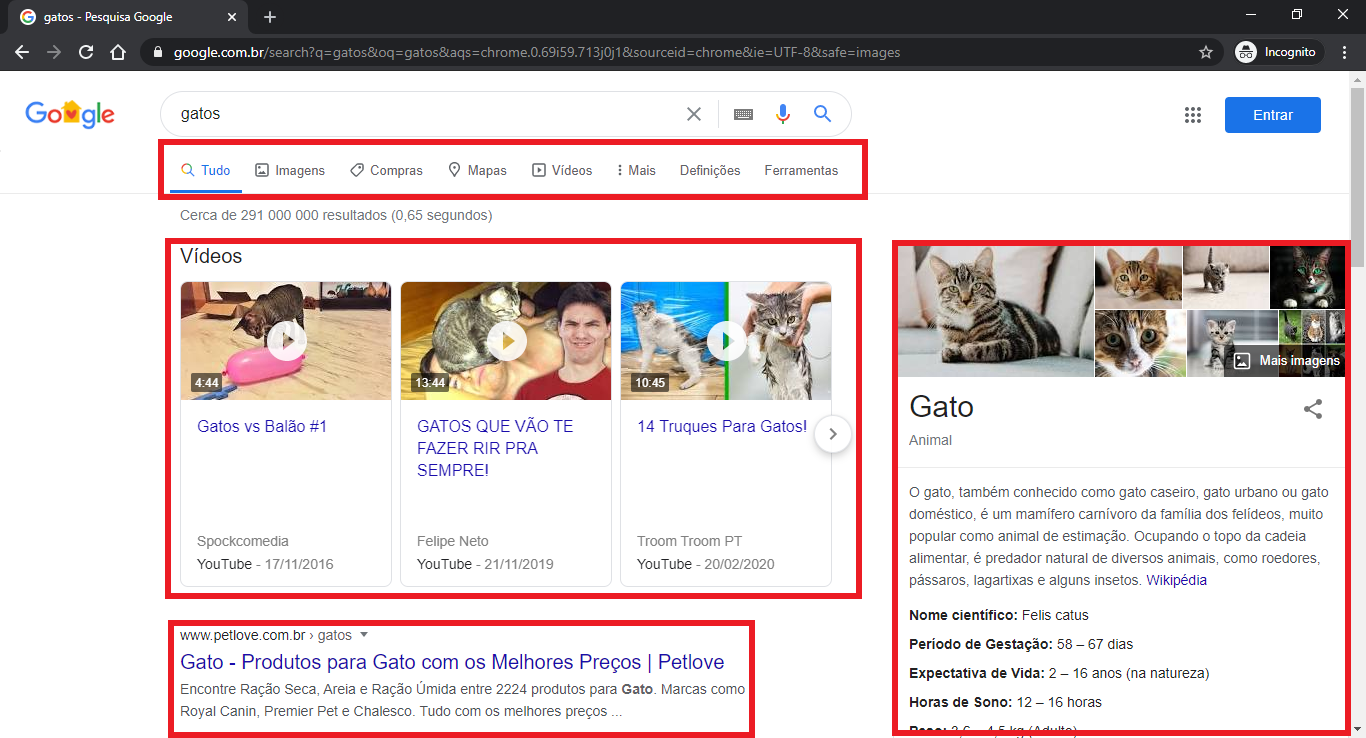
\includegraphics[width=0.75\linewidth]{Figuras/Ch03/fig2}
\end{frame}


\begin{frame}{Mecanismos de busca}
	\begin{block}{Utilidade}
		\begin{itemize}
			\item Podemos notar, então, que o conteúdo \textbf{não só} é \textbf{relacionado} ao que pesquisamos, como \textbf{também} está \textbf{hierarquizado}.
			\item Ou seja, mecanismos de busca também \textbf{processam o conteúdo exibido}, e aí vemos \textbf{informação} relacionada ao que pesquisamos.
			\item Tomemos outro exemplo, dessa vez, de algo que nós \textbf{não sabemos}.
			\item Digamos que, lendo um livro didático, você encontra uma \textbf{palavra desconhecida}, e não acha seu significado no livro: Quimera.
		\end{itemize}
	\end{block}

	%	\centering
	%	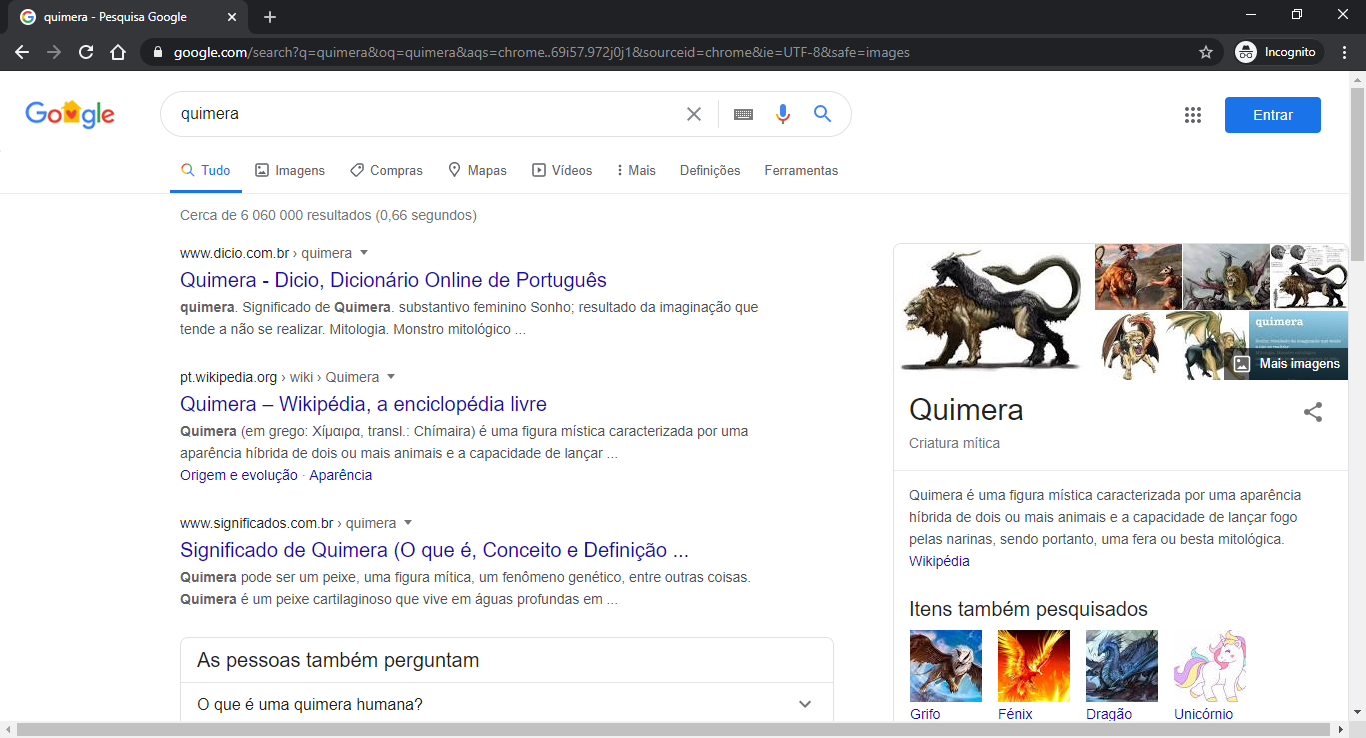
\includegraphics[width=0.7\linewidth]{Figuras/Ch03/fig3}
\end{frame}


\begin{frame}{Mecanismos de busca}

	\centering
	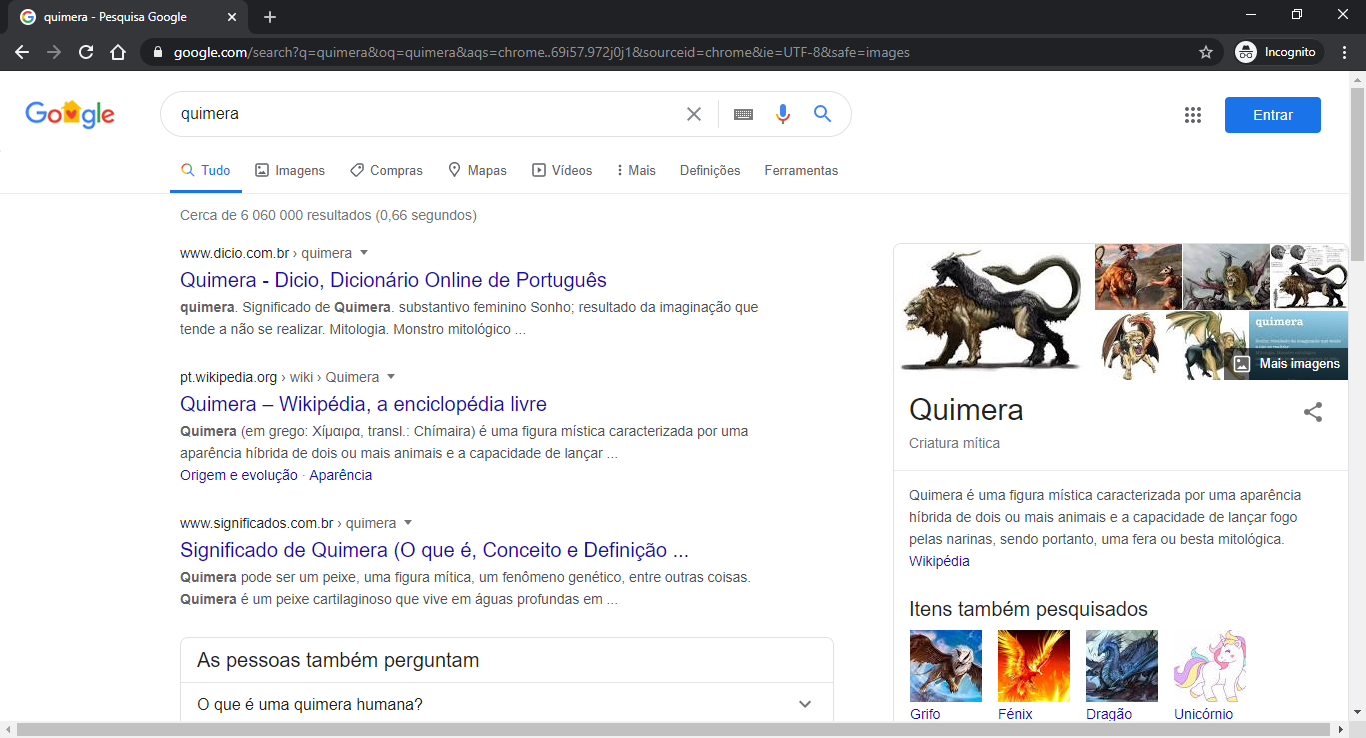
\includegraphics[width=1\linewidth]{Figuras/Ch03/fig3}
\end{frame}


\begin{frame}{Mecanismos de busca}
	\begin{block}{Utilidade}
		\begin{itemize}
			\item Repare que o Google fez algo \textbf{diferente} dessa vez.
			\item Ao invés de vídeos e fotos de quimeras, ele nos exibiu \textbf{verbetes de dicionário}, com a definição do que seria uma \textit{quimera}.
		\end{itemize}
	\end{block}

	\centering
	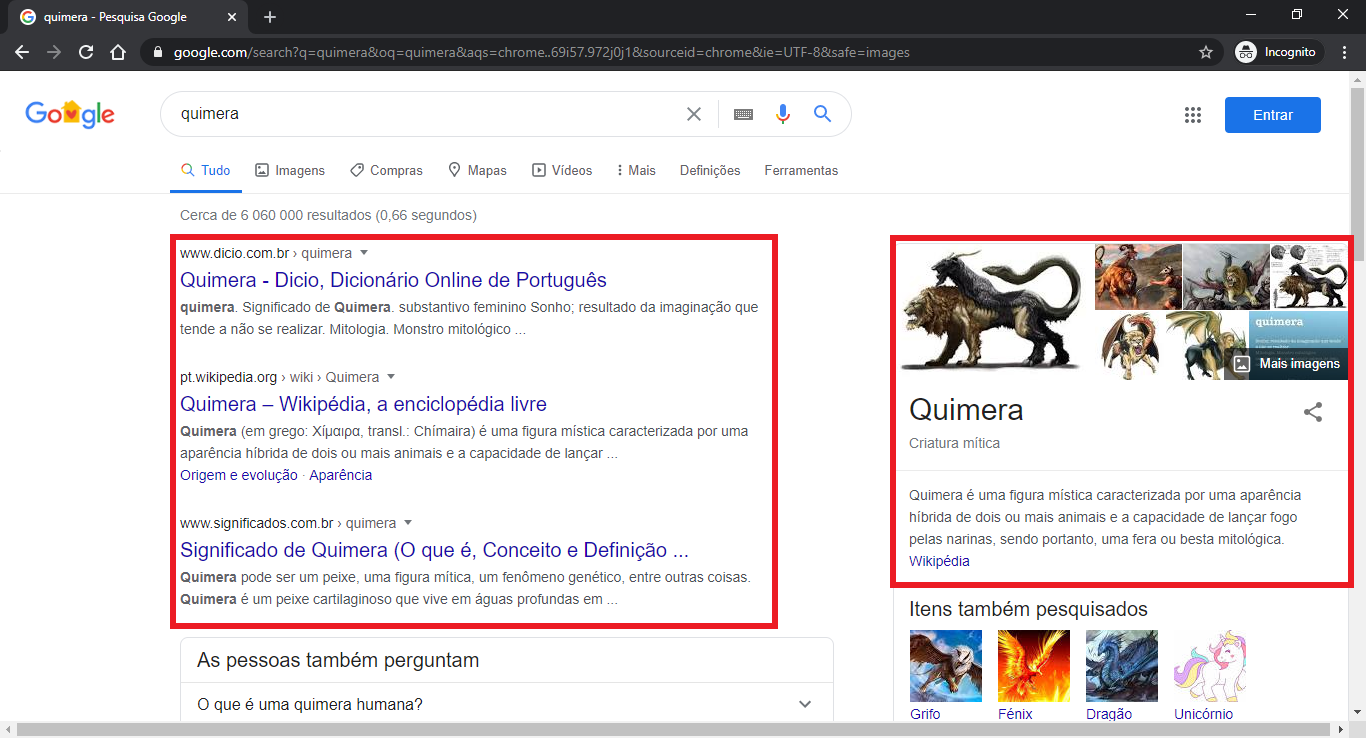
\includegraphics[width=0.8\linewidth]{Figuras/Ch03/fig4}
\end{frame}


\begin{frame}{Mecanismos de busca}
	\begin{block}{Funcionamento}
		Como o Google sabe o que desejamos?
		\begin{itemize}
			\item A resposta é bastante \textbf{complexa}, mas é basicamente um dos poderes do \textit{big data}.
			\item O Google analisa o que é útil para a \textbf{maioria das pessoas} que pesquisam ``quimera'' e, a partir daí, nos exibe o que ele \textbf{acha} que vai ser útil (obviamente ele também analisa \textbf{o seu comportamento \textit{online}}).
			\item Por exemplo, se a maioria das pessoas que pesquisa sobre gatos quer \textbf{ver vídeos} ou \textbf{comprar brinquedos} pros seus gatos, o Google tende a oferecer essas coisas.
			\item Porém, se você é um cientista que estuda mamíferos domesticados, talvez ele te mostre outros resultados...
		\end{itemize}
	\end{block}

	%	\centering
	%	\includegraphics[width=0.7\linewidth]{Figuras/Ch03/fig}
\end{frame}


\begin{frame}{Mecanismos de busca}
	\begin{block}{Funcionamento}
		Ainda é possível notar que os resultados tendem a ser coisas \textbf{mais recentes}, e também páginas \textbf{mais famosas}:
		\begin{itemize}
			\item Se muita gente \textbf{acessa }ou \textbf{cita} um determinado site de notícias, a probabilidade de que esse site tenha \textbf{conteúdo de qualidade }é maior e, portanto, o Google vai recomendá-lo.
		\end{itemize}
	\end{block}

	\centering
	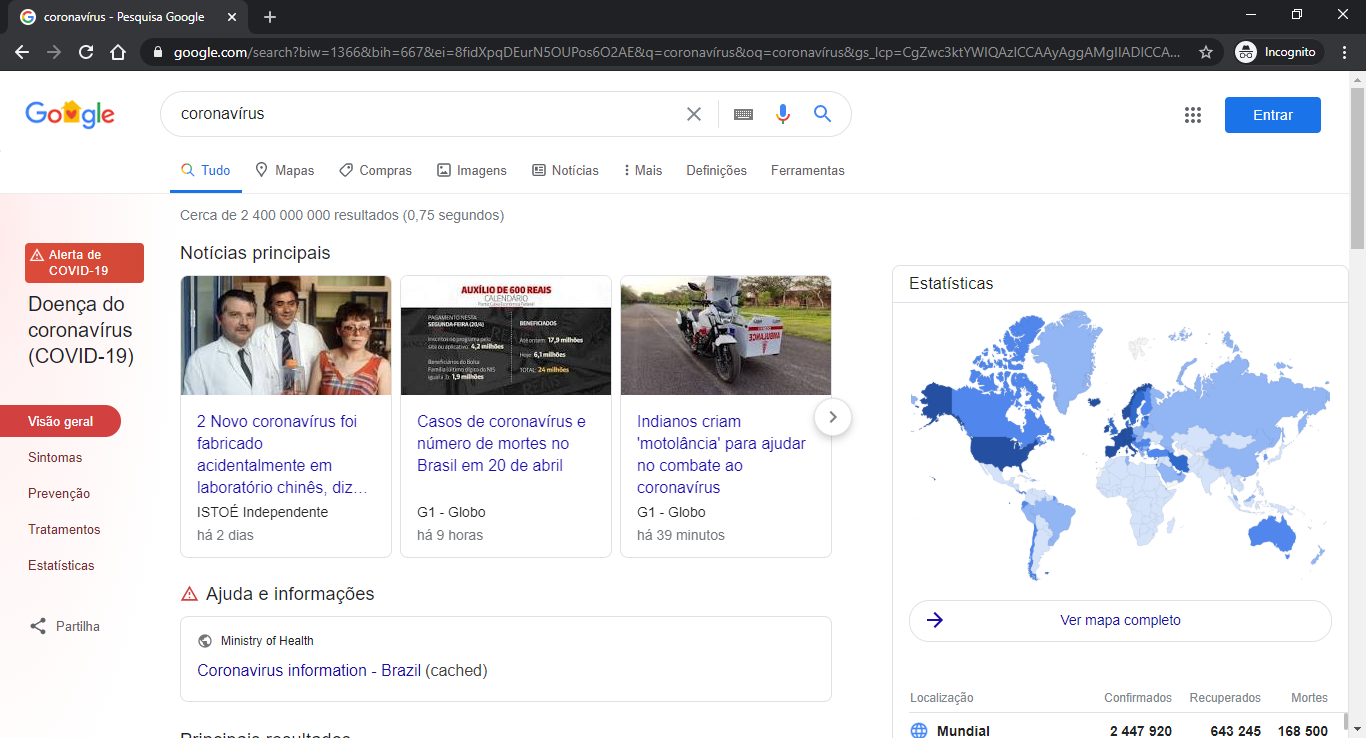
\includegraphics[width=0.7\linewidth]{Figuras/Ch03/fig5}
\end{frame}


\begin{frame}{Mecanismos de busca}
	\begin{block}{Funcionamento}
		\begin{itemize}
			\item No entanto, se formos nas páginas mais adiante, podemos encontrar resultados \textbf{estranhos}.
		\end{itemize}
	\end{block}

	\centering
	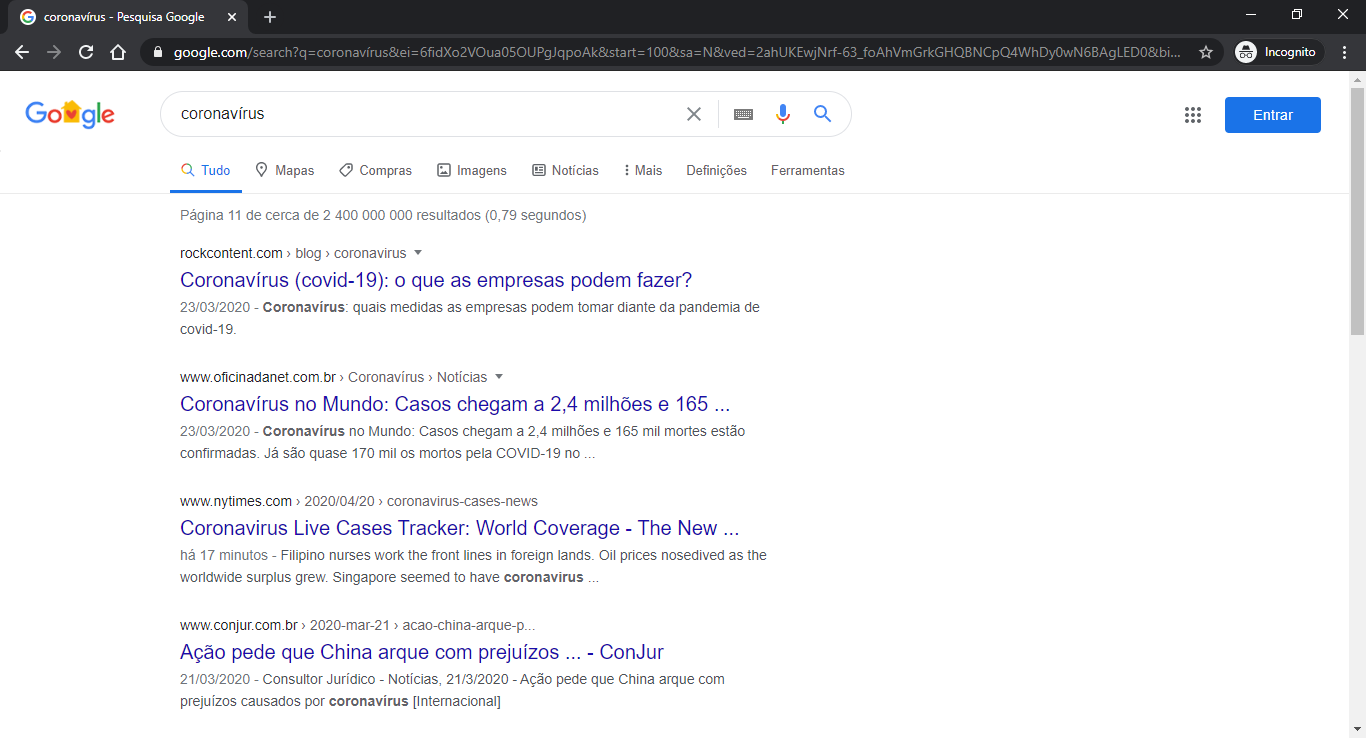
\includegraphics[width=0.9\linewidth]{Figuras/Ch03/fig6}
\end{frame}


\begin{frame}{Mecanismos de busca}
	\begin{block}{Filtragem}
		\begin{itemize}
			\item Por mais que o Google tenha milhares de resultados, vários são \textbf{omitidos}, pois podem ser muito \textbf{antigos}, \textbf{inadequados}, ou \textbf{repetidos}.
		\end{itemize}
	\end{block}

	\centering
	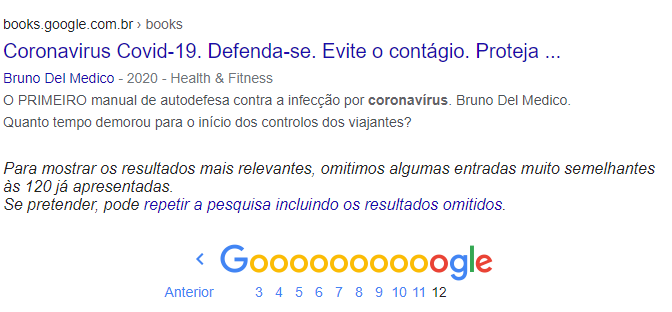
\includegraphics[width=0.9\linewidth]{Figuras/Ch03/fig7}
\end{frame}


\begin{frame}{Mecanismos de busca}
	\begin{block}{Métodos}
		\begin{itemize}
			\item Quando fazemos uma pesquisa na internet, devemos ter uma noção do que queremos:
			      \begin{itemize}
				      \item\normalsize Imagine que você viu uma coisa desconhecida numa conversa de \textit{Whatsapp}, por exemplo, alguém falou sobre ``Cosmologia''.
				      \item\normalsize Pelo assunto, podemos notar que é algo relacionado à física.
			      \end{itemize}
		\end{itemize}
	\end{block}

	\centering
	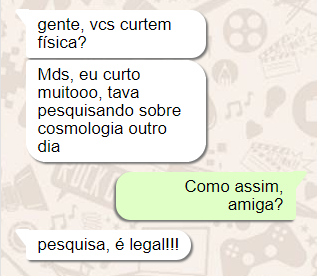
\includegraphics[width=0.45\linewidth]{Figuras/Ch03/fig7.4}
\end{frame}


\begin{frame}{Mecanismos de busca}
	\begin{block}{Métodos}
		\begin{itemize}
			\item Pesquisando, podemos ver o que é, e ter uma vaga noção sobre o que nossa amiga está falando, mas e se fosse necessário fazer um trabalho sobre o assunto?
			\item Nem sempre ler e copiar de um site é suficiente, pois é necessário \textbf{verificar as informações}.
		\end{itemize}
	\end{block}

	\centering
	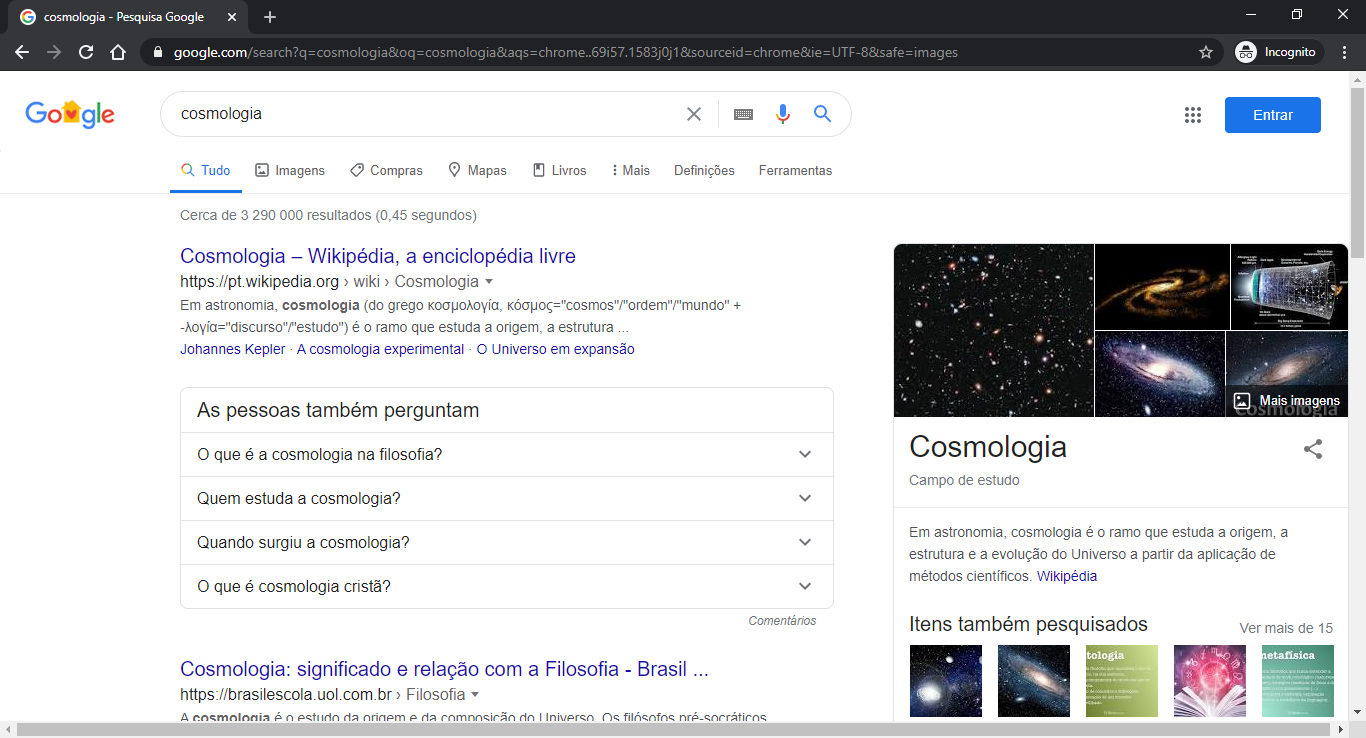
\includegraphics[width=0.7\linewidth]{Figuras/Ch03/fig7.5}
\end{frame}


\begin{frame}{Mecanismos de busca}
	\begin{block}{Métodos}
		\begin{itemize}
			\item Primeiro, podemos abrir um link da \textit{Wikipédia}, por exemplo, que é uma \textbf{enciclopédia virtual colaborativa}.
			\item Por ser uma enciclopédia, nem tudo está bem explicado, e alguns detalhes podem ser bastante \textbf{técnicos}, portanto não é uma boa fonte para \textbf{aprender} coisas.
			\item Além disso, ela é \textbf{colaborativa}, e isso faz com que algumas partes da entrada sejam bem detalhadas, e outras nem tanto, porque depende da boa vontade de cada um em completar (e quem sabe, algum dia você queira colaborar!)
		\end{itemize}
	\end{block}

	%	\centering
	%	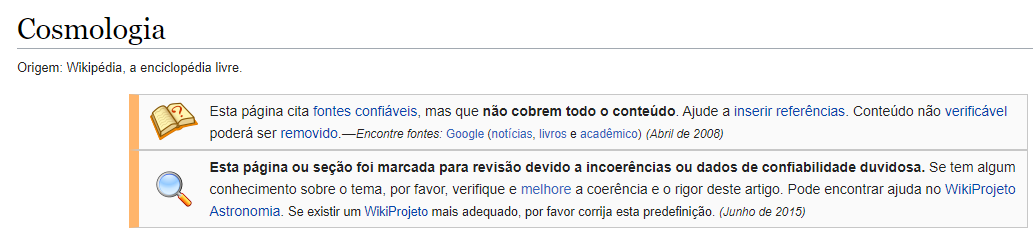
\includegraphics[width=0.7\linewidth]{Figuras/Ch03/fig7.6}
\end{frame}


\begin{frame}{Mecanismos de busca}
	\begin{block}{Métodos}
		\begin{itemize}
			\item Ao abrir a página já podemos ver um aviso sobre as possíveis incoerências:
		\end{itemize}
	\end{block}

	\centering
	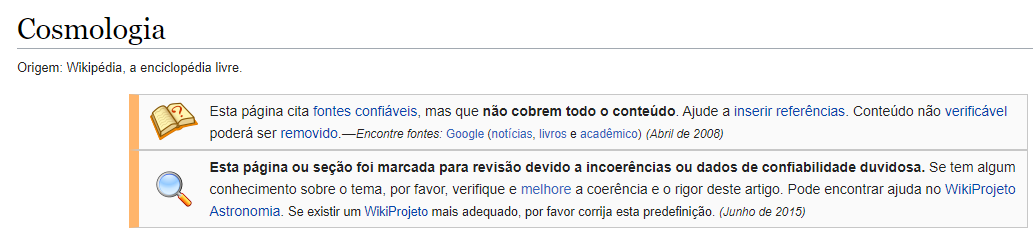
\includegraphics[width=1\linewidth]{Figuras/Ch03/fig7.6}
\end{frame}


\begin{frame}{Mecanismos de busca}
	\begin{block}{Métodos}
		\begin{itemize}
			\item Uma coisa muito útil sobre a Wiki, é que podemos olhar o \textbf{índice} para ter uma noção dos \textbf{tópicos} do assunto, e ter alguma ideia de \textbf{como estruturar um trabalho}.
		\end{itemize}
	\end{block}

	\centering
	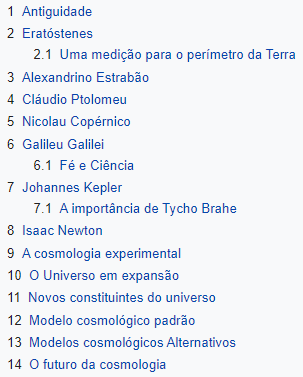
\includegraphics[width=0.36\linewidth]{Figuras/Ch03/fig7.7}
\end{frame}


\begin{frame}{Mecanismos de busca}
	\begin{block}{Métodos}
		\begin{itemize}
			\item A partir daí podemos procurar \textbf{cada um dos tópicos} em sites separados, ou então olhar outros \textbf{índices} para conferir se a Wiki abordou o assunto em sua completude.
			\item Por exemplo, o pdf abaixo parece ser uma boa fonte para aprender sobre o assunto.
		\end{itemize}
	\end{block}

	\centering
	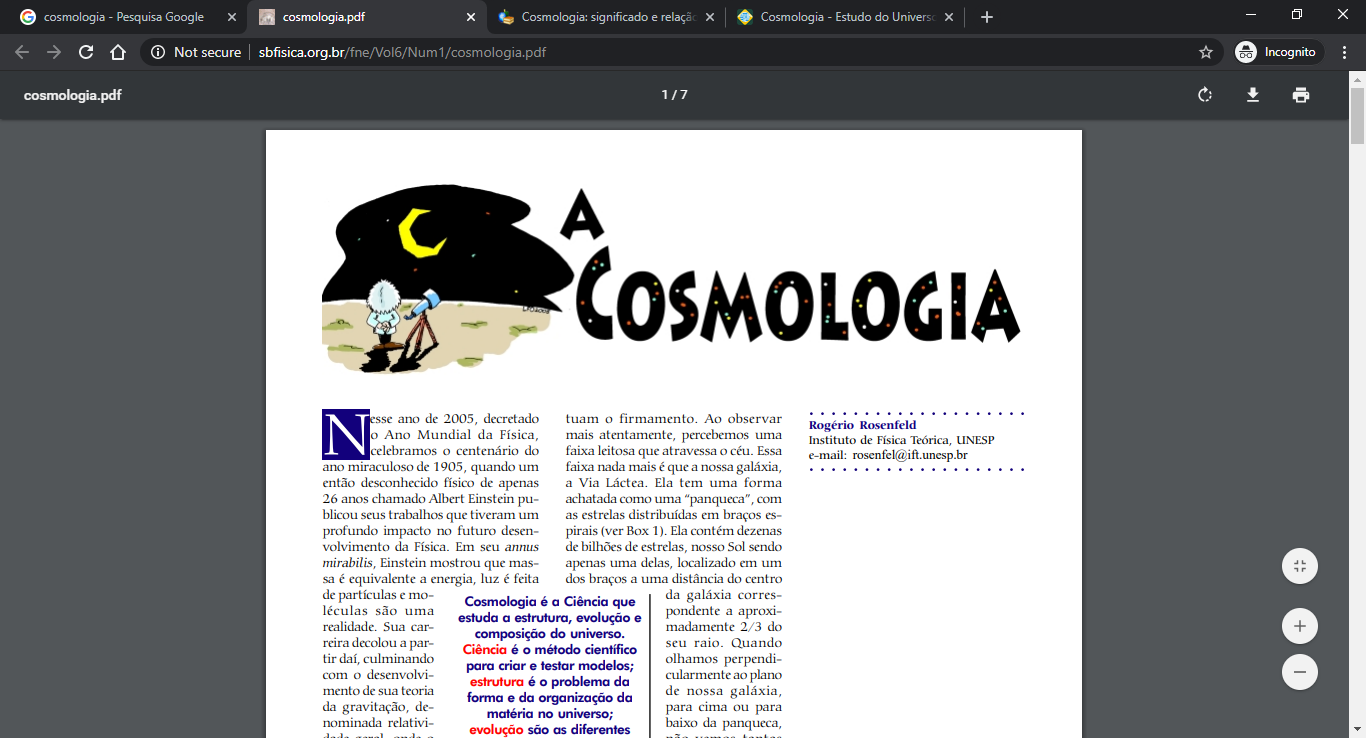
\includegraphics[width=0.7\linewidth]{Figuras/Ch03/fig7.8}
\end{frame}


\begin{frame}{Mecanismos de busca}
	\begin{block}{Métodos}
		\begin{itemize}
			\item Podemos verificar \textbf{boas fontes} por dois critérios:
			      \begin{itemize}
				      \item\normalsize \textbf{Quem escreveu?} (Professor, estudante, etc).
				      \item\normalsize \textbf{Onde está?} (Site pessoal, site de notícias, etc).
			      \end{itemize}
			\item Uma ótima ferramenta é pesquisar \textbf{em inglês}, pois há \textbf{mais conteúdo} e também há \textbf{conteúdos melhores}, dependendo do que pesquisamos.
			\item Seu método para uma \textbf{boa pesquisa }surgirá com a \textbf{experiência}, e isso conseguimos através do \textbf{esforço} e da \textbf{prática}.
		\end{itemize}
	\end{block}

	%	\centering
	%	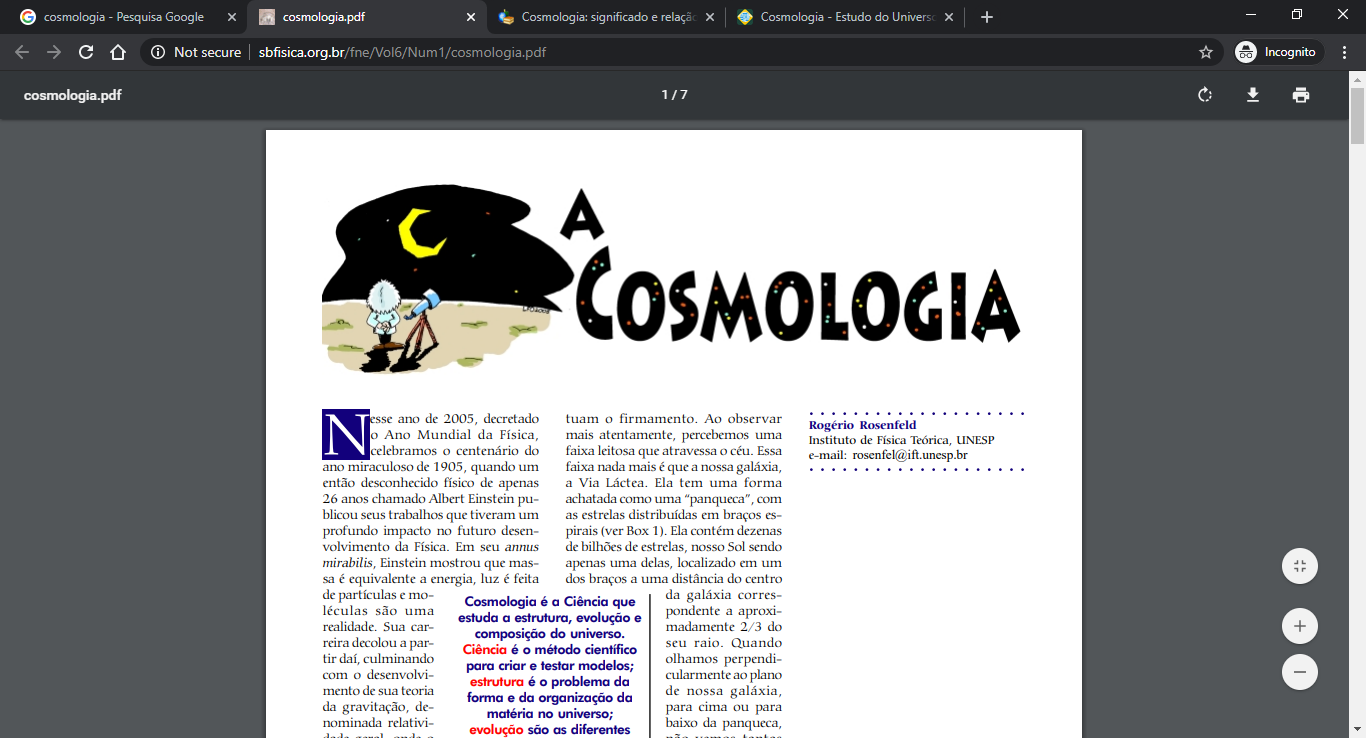
\includegraphics[width=0.7\linewidth]{Figuras/Ch03/fig7.8}
\end{frame}


\begin{frame}{Mecanismos de busca}
	\begin{block}{Acesso ao conteúdo}
		\begin{itemize}
			\item Se você usa bastante a internet, sabe que quase todo o conteúdo que acessamos está num site \textbf{conhecido}, ou que podemos achar pelo Google.
			\item Porém, isso não representa toda a internet, e existem estimativas que dizem que \textbf{só conseguimos acessar 4\% da internet }usando um mecanismo de busca \textbf{convencional }(Google, Bing, Yahoo, etc).
			\item E onde está ``o resto'' da internet?
			\item Simplesmente, está \textbf{escondida} dos usuários normais, na \textit{deep web} e na \textit{dark web}.
		\end{itemize}
	\end{block}

	%	\centering
	%	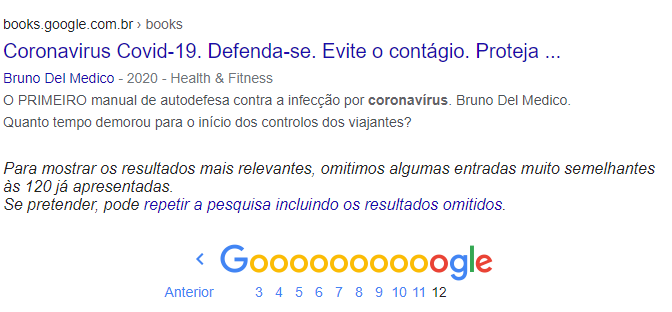
\includegraphics[width=0.7\linewidth]{Figuras/Ch03/fig7}
\end{frame}


\begin{frame}{Mecanismos de busca}
	\centering
	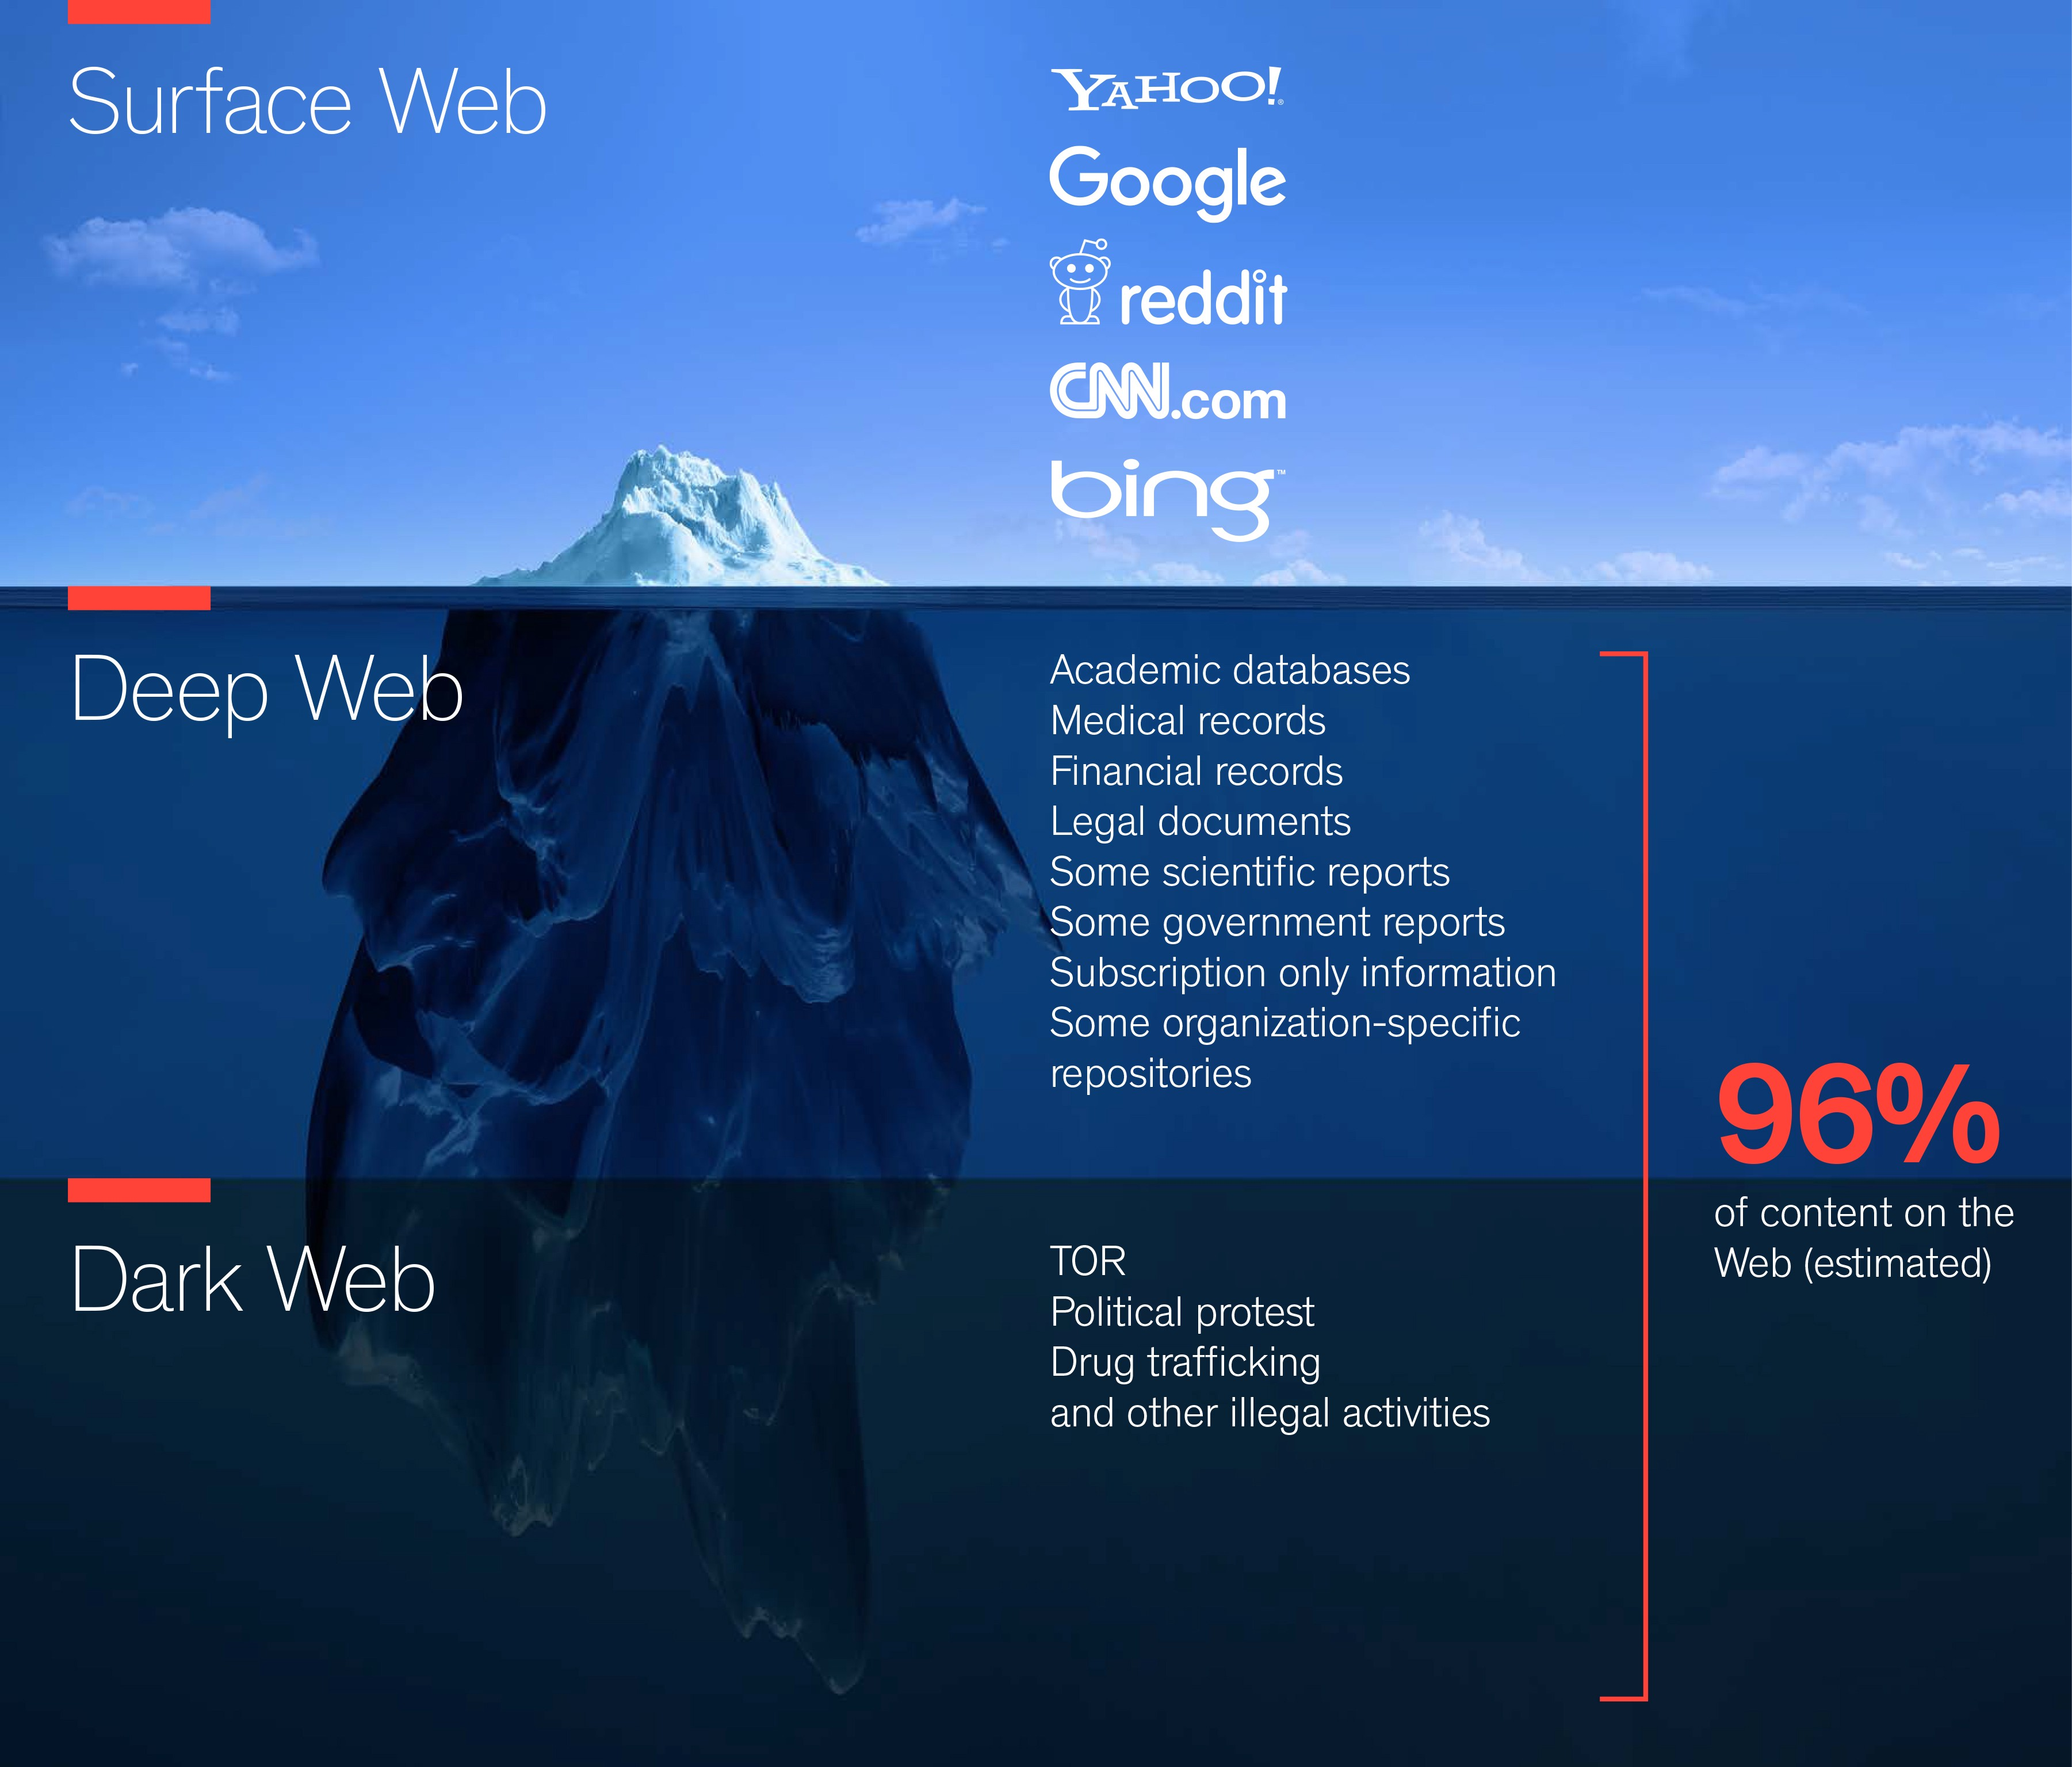
\includegraphics[width=0.7\linewidth]{Figuras/Ch03/fig8}
\end{frame}


\begin{frame}{Mecanismos de busca}
	\begin{block}{Camadas}
		Essas ``camadas'' mais profundas da internet são \textbf{inacessíveis} pois contém \textbf{conteúdo privado} --- que pertence a empresas ou a indivíduos --- ou \textbf{conteúdo ilícito}, que não pode ser facilmente erradicado, por duas razões:
		\begin{itemize}
			\item legislações locais, que não dão autonomia para desligar um pedaço da internet;
			\item dificuldade em apontar exatamente \textbf{onde} o conteúdo está hospedado.
		\end{itemize}
	\end{block}

	%	\centering
	%	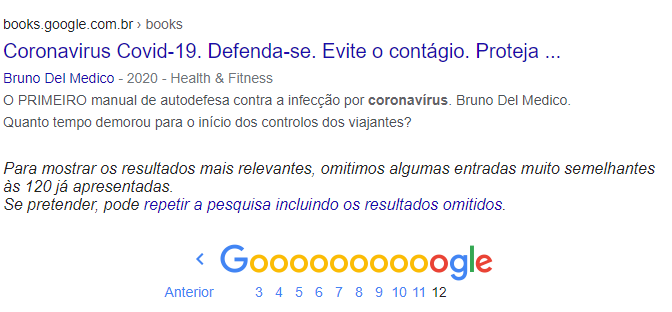
\includegraphics[width=0.7\linewidth]{Figuras/Ch03/fig7}
\end{frame}


\begin{frame}{Internet}
	\begin{block}{Introdução}
		\begin{itemize}
			\item Para entendermos melhor como funciona tudo isso, é necessário dar um passo atrás para entender exatamente \textbf{o que} é a internet: como é composta, como funciona, como a acessamos, dentre outros detalhes.
			\item Primeiro, precisamos discutir suas \textbf{origens}, que datam dos anos 60.
		\end{itemize}
	\end{block}

	\centering
	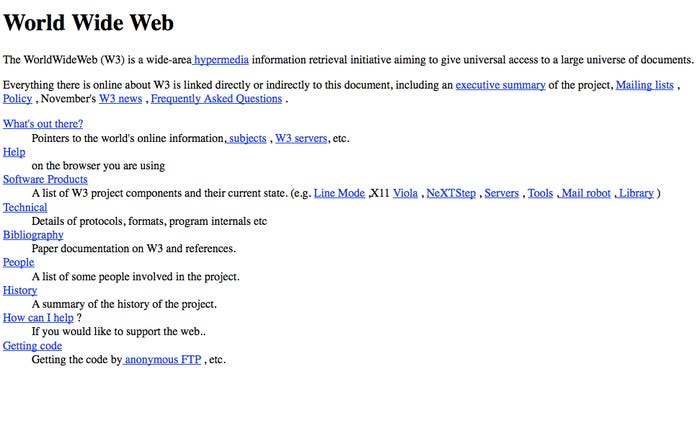
\includegraphics[width=0.75\linewidth]{Figuras/Ch03/fig7.2}
\end{frame}


\begin{frame}{Internet}
	\begin{block}{Origem}
		\begin{itemize}
			\item O propósito inicial da ``internet'', era ser uma ferramenta de \textbf{compartilhamento de recursos} entre computadores e, nos anos 60, a ideia era que os computadores seriam, para sempre, grandes cérebros que trabalham para indústrias, bancos e fins militares.
			\item Desse modo, grandes matemáticos se envolveram no processo, numa iniciativa do departamento de defesa dos EUA, chamada \textsmaller{\textbf{ARPANET}}.
			\item A ideia era criar \textbf{protocolos} para a troca de informações remotamente, numa \textbf{rede interconectada}.
			\item Internet = Inter (entre) + net (que vem de \textit{network}, ou rede).
			\item No início, eram necessárias \textbf{conexões diretas} com quem se queria compartilhar informações, devendo haver um \textbf{protocolo mútuo} para a troca de dados.
			\item Com o advento de protocolos normalizados, como o TCP/IP, \textbf{qualquer um} poderia usar a internet.
		\end{itemize}
	\end{block}

	%	\centering
	%	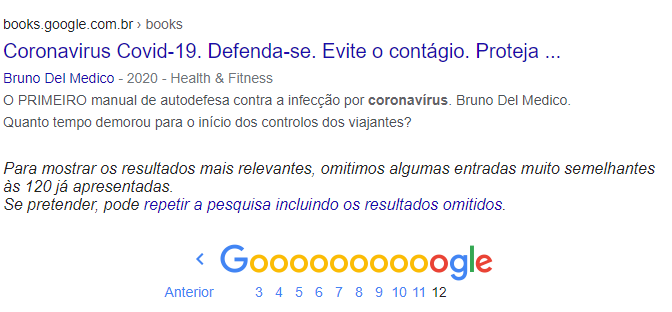
\includegraphics[width=0.7\linewidth]{Figuras/Ch03/fig7}
\end{frame}


\begin{frame}{Internet}
	\begin{block}{Origem}
		\begin{itemize}
			\item Os \textbf{sites}, então, começaram a surgir quando mais computadores se conectaram à rede.
			\item Esses sites eram meramente uma \textbf{parte acessível} dos computadores que se conectavam, e estava disponível para os demais usuários.
			\item A medida que os sites crescem, e o número de usuários também, é \textbf{inviável} compartilhar parte de um computador para acesso, e são necessários \textbf{servidores}.
			\item Os servidores são grandes \textbf{depósitos}, com enorme capacidade de \textbf{troca de dados}, onde ficam \textbf{hospedados} os sites e serviços que utilizamos.
		\end{itemize}
	\end{block}

	%	\centering
	%	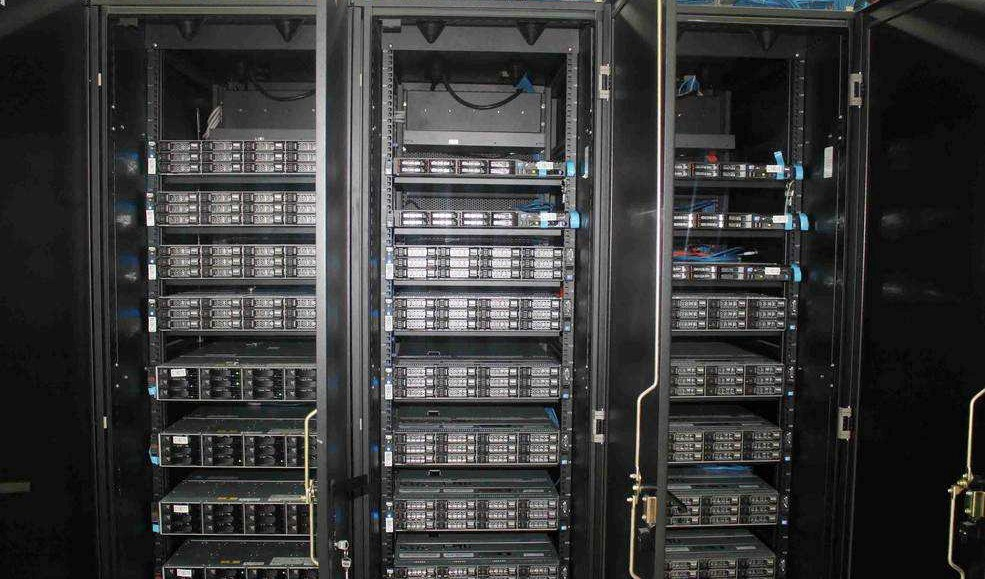
\includegraphics[width=0.7\linewidth]{Figuras/Ch03/fig7.3}
\end{frame}


\begin{frame}{Internet}

	\centering
	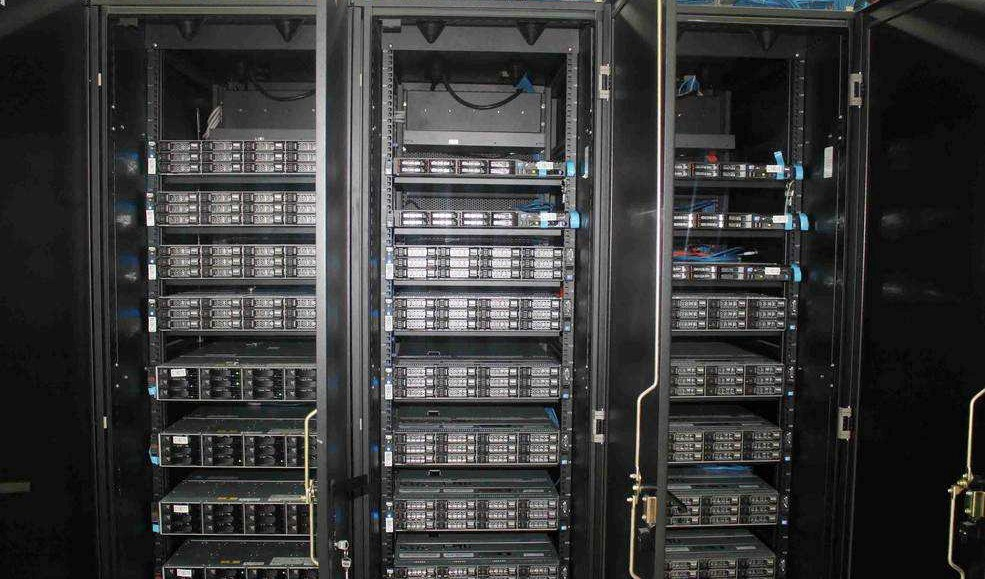
\includegraphics[width=1\linewidth]{Figuras/Ch03/fig7.3}
\end{frame}


\begin{frame}{Servidores}
	\begin{block}{Acesso}
		\begin{itemize}
			\item Para acessar um site, utilizamos um \textbf{endereço IP}, próprio daquele site.
			\item Todos os seus dispositivos tem IP's próprios, e são eles que identificam \textbf{quem é quem} na rede.
			\item Os IP's de sites podem ser acessados pelo \textbf{DNS}, que é um grande \textbf{catálogo} de \textbf{nomes} com \textbf{endereços correspondentes}.
			\item O Google, por exemplo, possui os IP's 172.217.0.0 -- 172.217.31.255.
			\item Se digitarmos algum desses endereços no navegador, somos levados ao site.
		\end{itemize}
	\end{block}

	\centering
	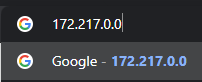
\includegraphics[width=0.5\linewidth]{Figuras/Ch03/fig9}
\end{frame}


\begin{frame}{Servidores}
	\begin{block}{VPN's}
		\begin{itemize}
			\item Como mencionamos antes, só temos acesso a essa parte mais \textbf{superficial} da internet.
			\item Isso ocorre pois os sites que utilizamos possuem servidores disponíveis \textbf{abertamente}.
			\item Porém, para acessar a \textit{deep web} ou a \textit{dark web}, precisamos de acesso a \textbf{servidores anônimos}, que são capazes de \textbf{mascarar os IP}'s dos sites (e você deveria mascarar o seu também!)
			\item Esse anonimato é possível através de um \textbf{VPN}, por exemplo.
			\item Essa ferramenta acessa a internet de um \textbf{local diferente} de onde você está, e esse desvio permite que você se esconda: como um \textbf{muro}.
		\end{itemize}
	\end{block}

	%	\centering
	%	\includegraphics[width=0.7\linewidth]{Figuras/Ch03/fig}
\end{frame}


\begin{frame}{Servidores}
	\centering
	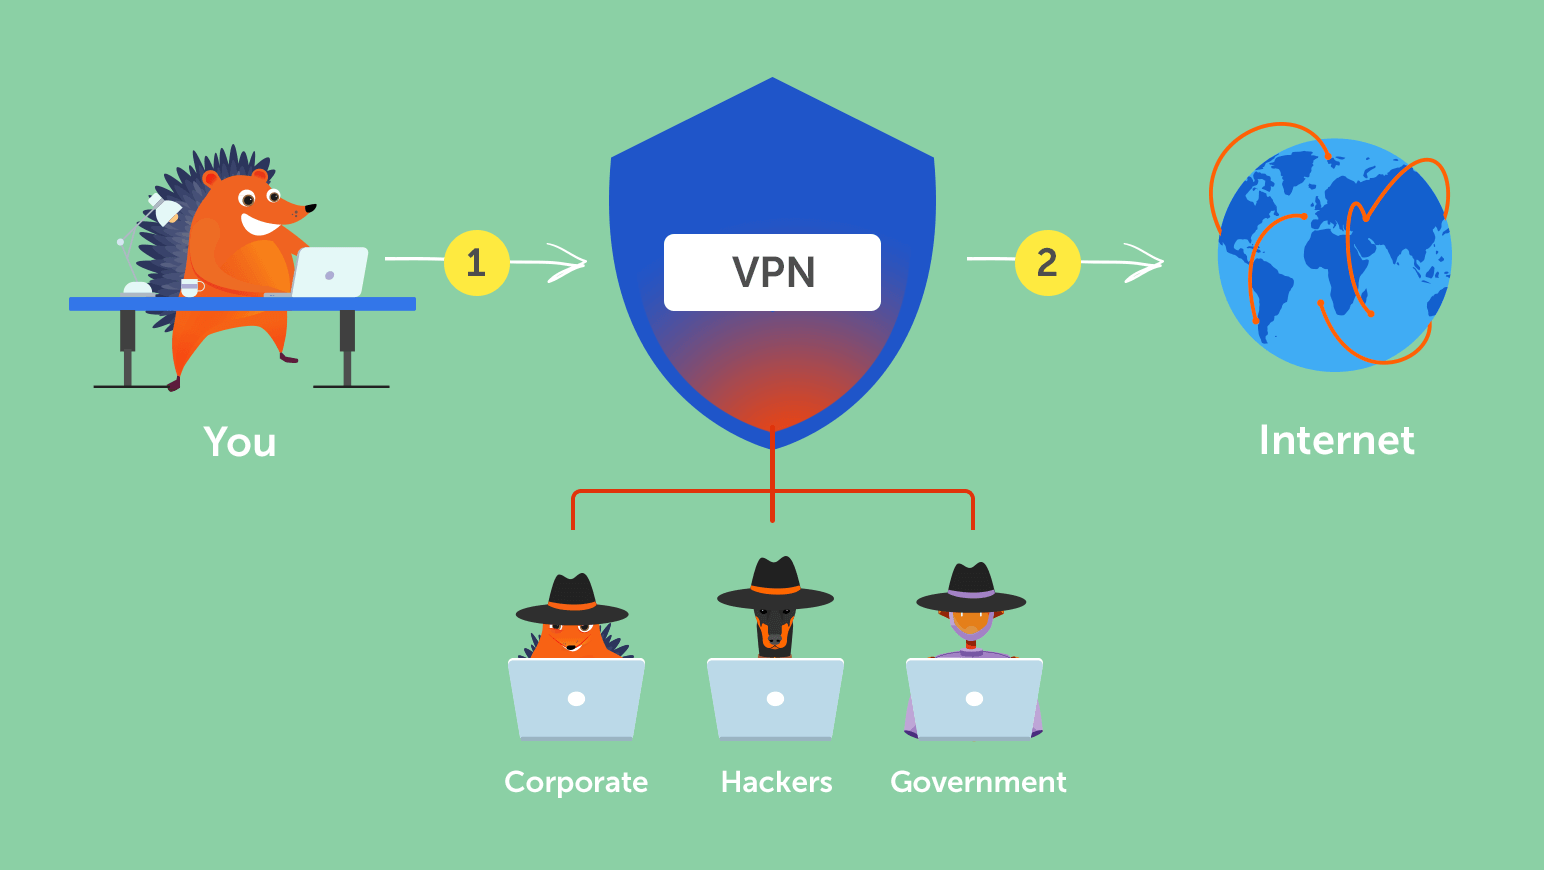
\includegraphics[width=1\linewidth]{Figuras/Ch03/fig10}
\end{frame}


\begin{frame}{Navegadores}
	\begin{block}{Introdução}
		\begin{itemize}
			\item Navegadores são ferramentas para acessar a internet.
			\item Geralmente utilizamos o Google Chrome, Mozilla Firefox, Safari ou Opera para acessar a internet de nossos computadores ou smartphones.
			\item O \textit{Google Chrome} (abaixo) é um dos navegadores mais \textbf{famosos}, e mais \textbf{utilizados}, e isso se deve à fama do \textit{Google}.
		\end{itemize}
	\end{block}

	\centering
	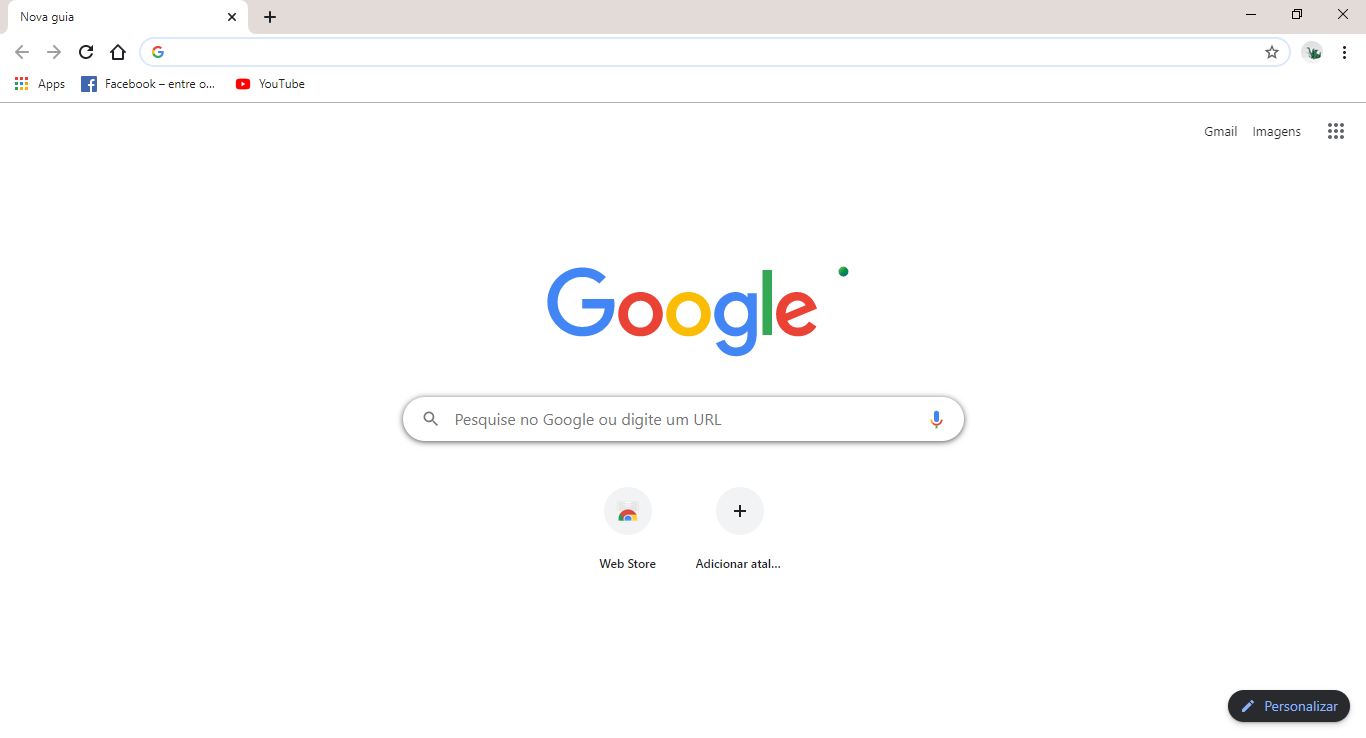
\includegraphics[width=0.7\linewidth]{Figuras/Ch03/fig8.2}
\end{frame}


\begin{frame}{Navegadores}
	\begin{block}{Google Chrome}
		Em sua janela podemos ver diversos elementos, como:
		\begin{enumerate}
			\item gerenciador de abas ou guias;
		\end{enumerate}
	\end{block}
	
	\centering
	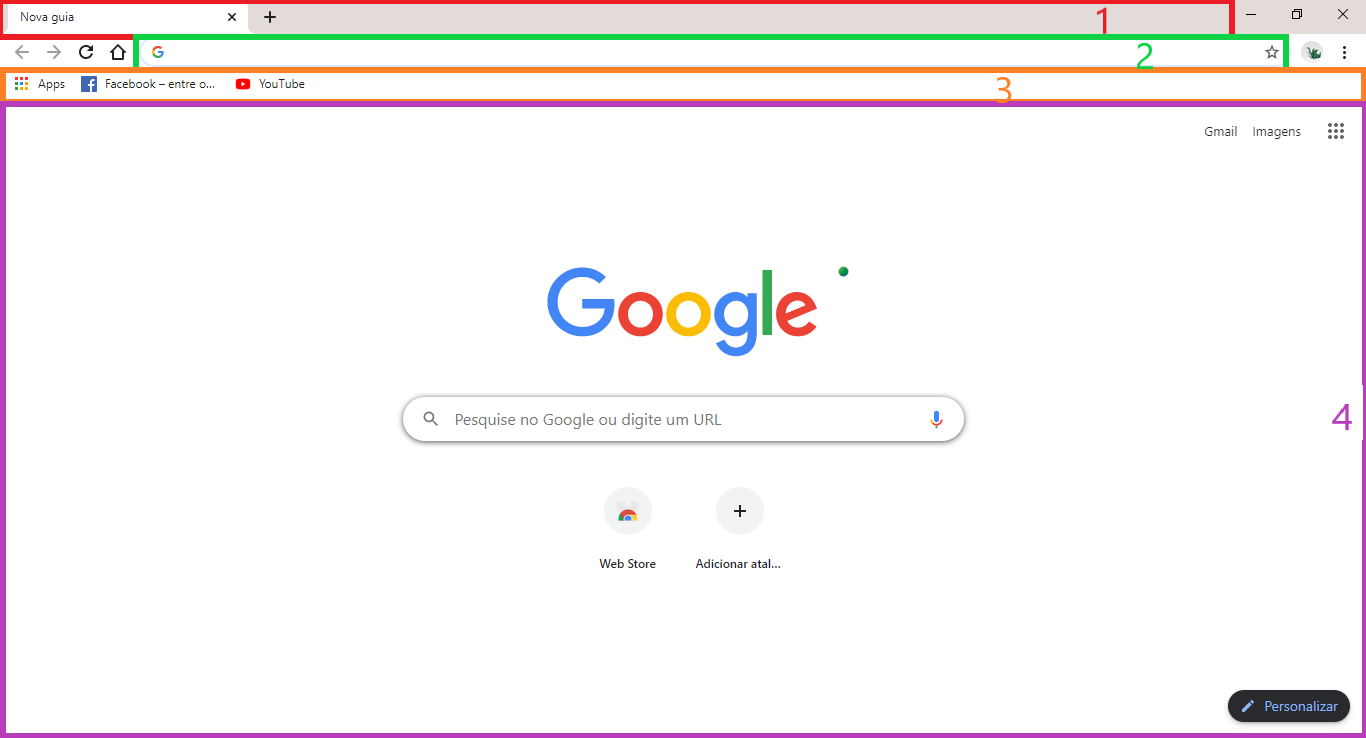
\includegraphics[width=0.8\linewidth]{Figuras/Ch03/fig8.6}
\end{frame}


\begin{frame}{Navegadores}
	\begin{block}{Google Chrome}
		\begin{enumerate}
			\setcounter{enumi}{1}
			\item barra de pesquisa;
		\end{enumerate}
	\end{block}
	
	\centering
	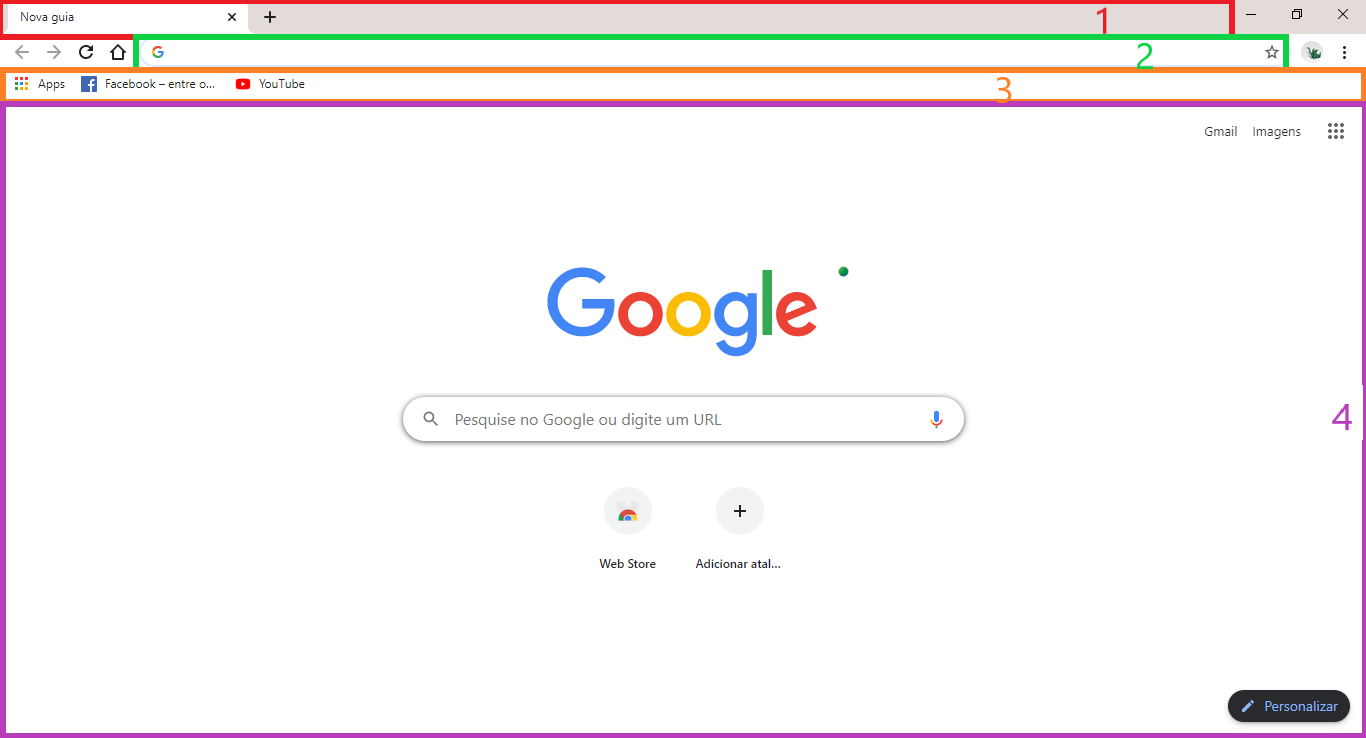
\includegraphics[width=0.9\linewidth]{Figuras/Ch03/fig8.6}
\end{frame}


\begin{frame}{Navegadores}
	\begin{block}{Google Chrome}
		\begin{enumerate}
			\setcounter{enumi}{2}
			\item barra de favoritos;
		\end{enumerate}
	\end{block}
	
	\centering
	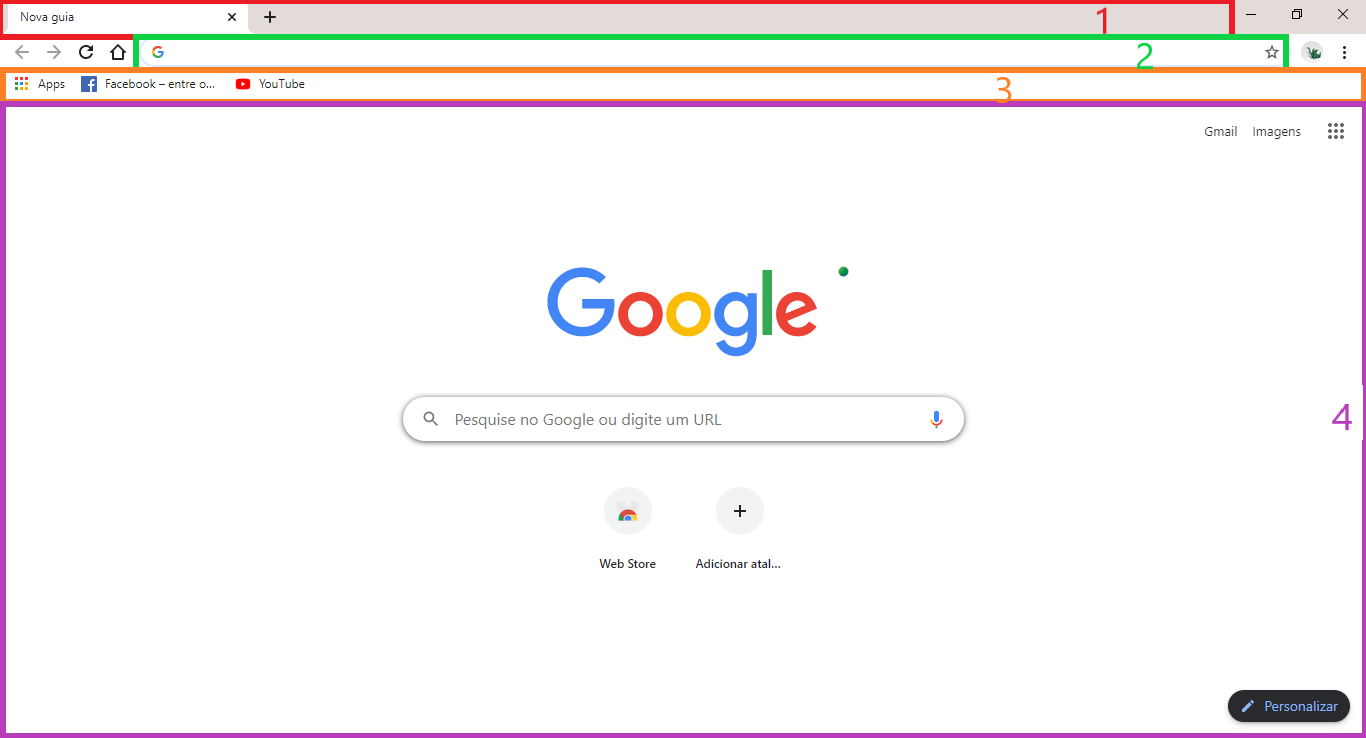
\includegraphics[width=0.9\linewidth]{Figuras/Ch03/fig8.6}
\end{frame}


\begin{frame}{Navegadores}
	\begin{block}{Google Chrome}
		\begin{enumerate}
			\setcounter{enumi}{3}
			\item janela de exibição.
		\end{enumerate}
	\end{block}
	
	\centering
	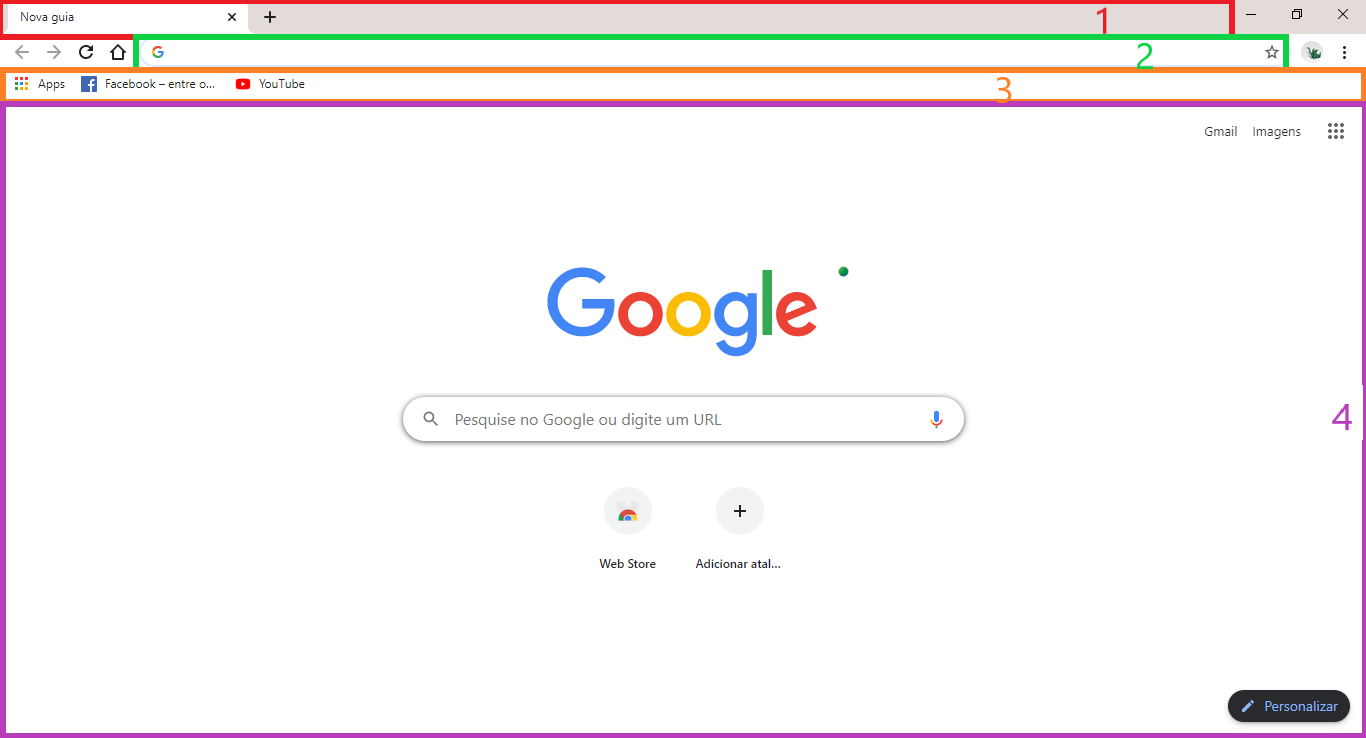
\includegraphics[width=0.9\linewidth]{Figuras/Ch03/fig8.6}
\end{frame}


\begin{frame}{Navegadores}
	\begin{block}{Google Chrome}
		\begin{itemize}
			\item Na barra de navegação há outras opções, como as \textbf{setas}, que permitem \textbf{navegar} entre as \textbf{páginas acessadas por uma guia}.
			\item A bolinha serve para \textbf{recarregar} uma página, o que é um recurso útil caso haja algum \textbf{problema} com o \textbf{site} ou com a \textbf{conexão}
			\item A \textbf{casinha} (home) nos dirige à uma \textbf{página específica} (personalizável), que pode ser de \textbf{frequente acesso}.
		\end{itemize}
	\end{block}
	
	\centering
	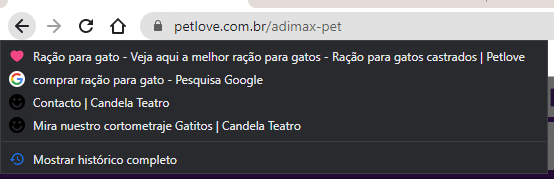
\includegraphics[width=0.9\linewidth]{Figuras/Ch03/fig8.10}
\end{frame}


\begin{frame}{Navegadores}
	\begin{block}{Google Chrome}
		\begin{itemize}
			\item No outro lado da barra, podemos \textbf{favoritar a página} clicando na \textbf{estrelinha}.
			\item Também podemos acessar as \textbf{configurações do navegador}, entre outras coisas, como \textbf{gerenciador de downloads}, ou o gerenciador de \textbf{favoritos}.
		\end{itemize}
	\end{block}
	
	\centering
	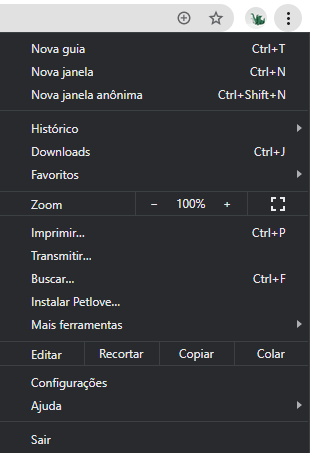
\includegraphics[width=0.25\linewidth]{Figuras/Ch03/fig8.11}
\end{frame}


\begin{frame}{Navegadores}
	\begin{block}{Google Chrome}
		\begin{itemize}
			\item Gerenciador de favoritos e guias abertas.
		\end{itemize}
	\end{block}
	
	\centering
	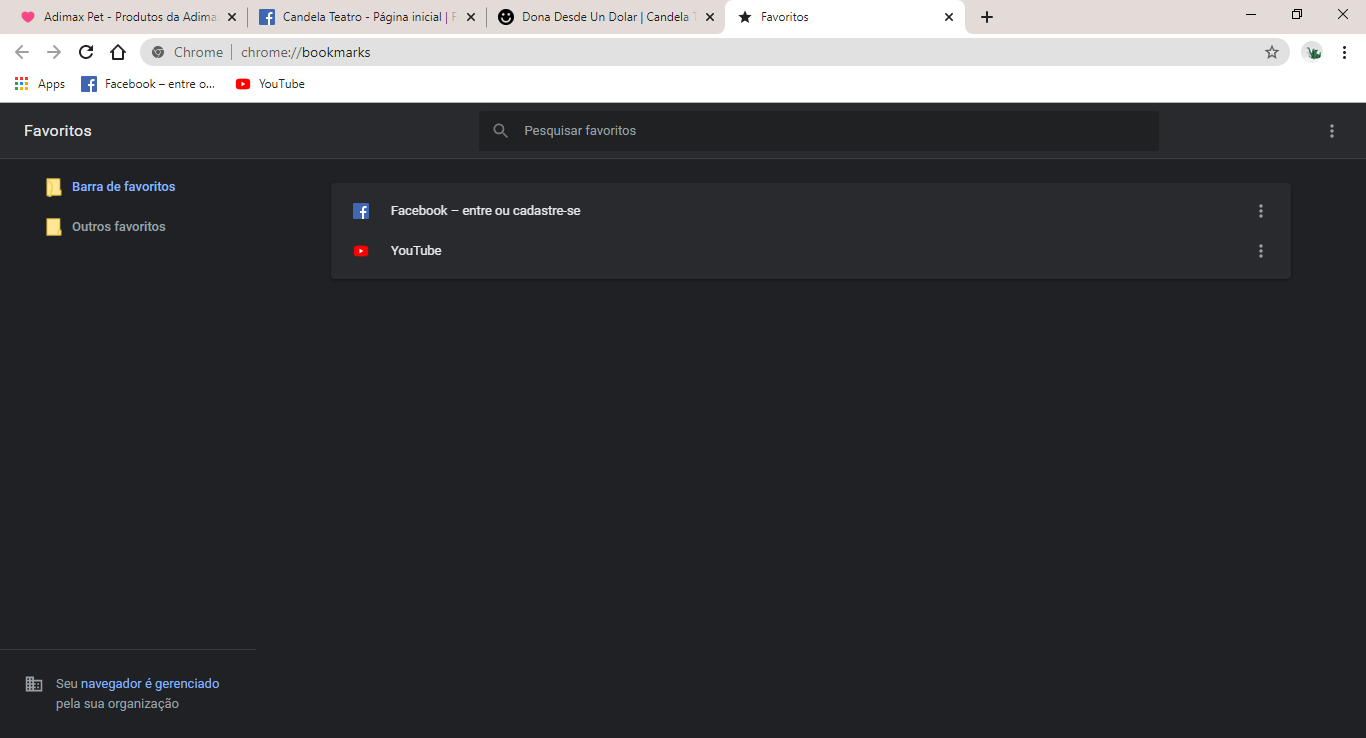
\includegraphics[width=0.9\linewidth]{Figuras/Ch03/fig8.12}
\end{frame}


\begin{frame}{Navegadores}
	\begin{block}{Google Chrome}
		\begin{itemize}
			\item Além disso, também podemos ver um \textbf{histórico de navegação}.
		\end{itemize}
	\end{block}
	
	\centering
	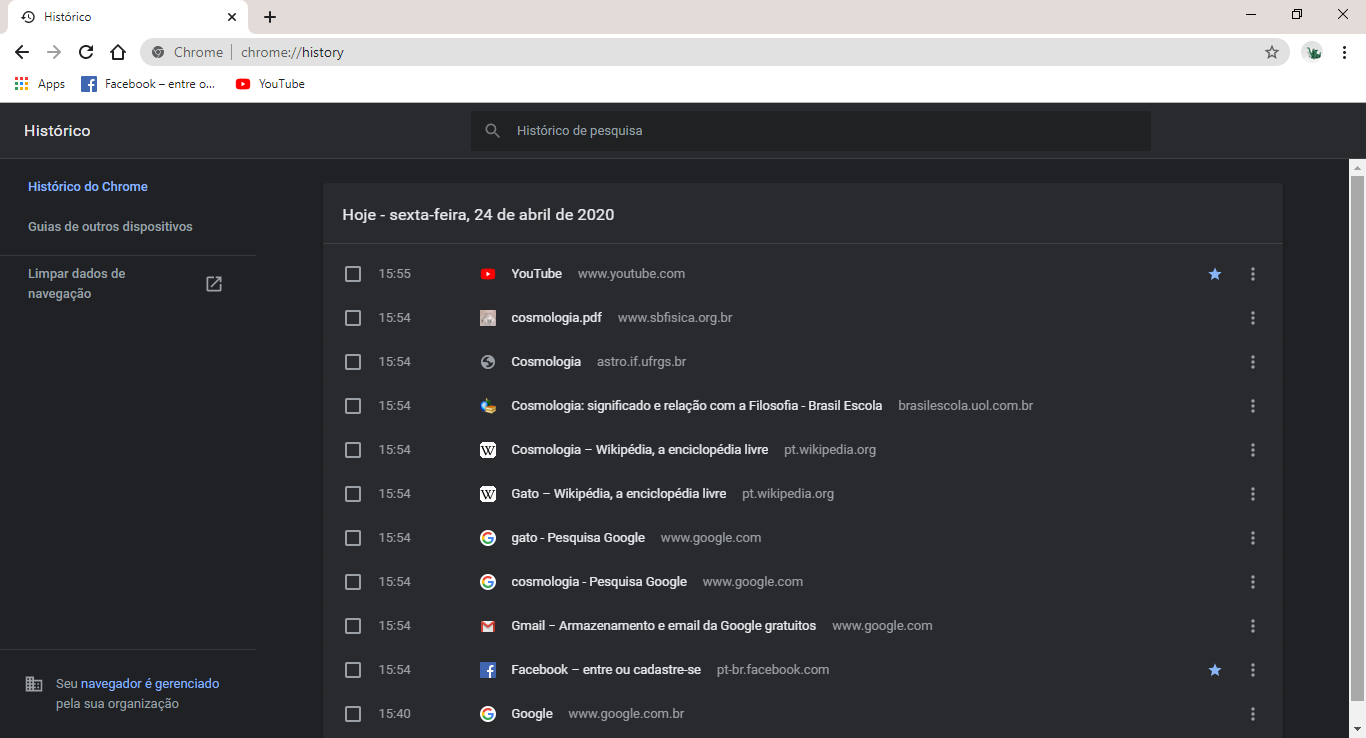
\includegraphics[width=0.9\linewidth]{Figuras/Ch03/fig8.8}
\end{frame}


\begin{frame}{Navegadores}
	\begin{block}{Google Chrome}
		\begin{itemize}
			\item E também temos acesso a \textbf{navegação anônima}, que nos permite navegar sem que nada seja \textbf{registrado} no computador.
		\end{itemize}
	\end{block}
	
	\centering
	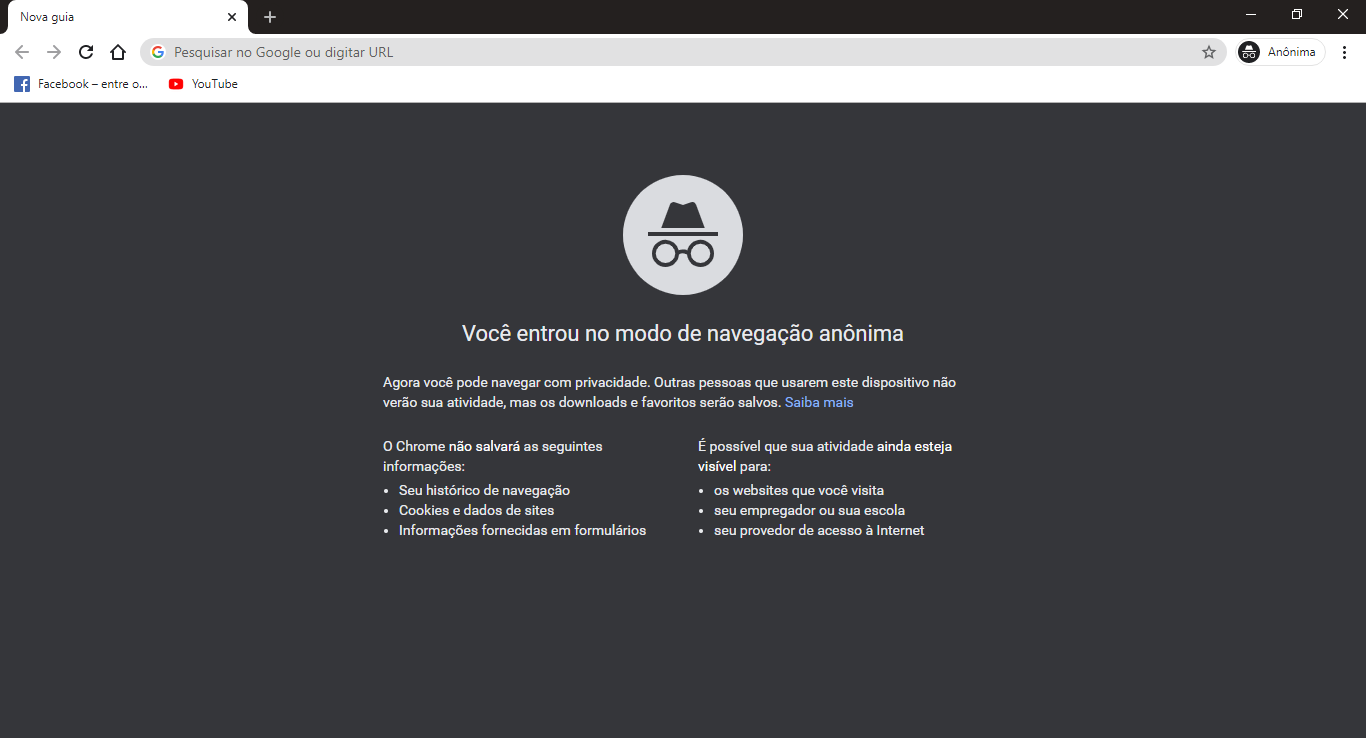
\includegraphics[width=0.9\linewidth]{Figuras/Ch03/fig8.7}
\end{frame}


\begin{frame}{Navegadores}
	\begin{block}{Google Chrome}
		\begin{itemize}
			\item Uma função interessante é o \textbf{autopreenchimento}, que permite que o navegador \textbf{preencha informações} para você, como \textbf{login}, ou \textbf{dados de pagamento}.
		\end{itemize}
	\end{block}
	
	\centering
	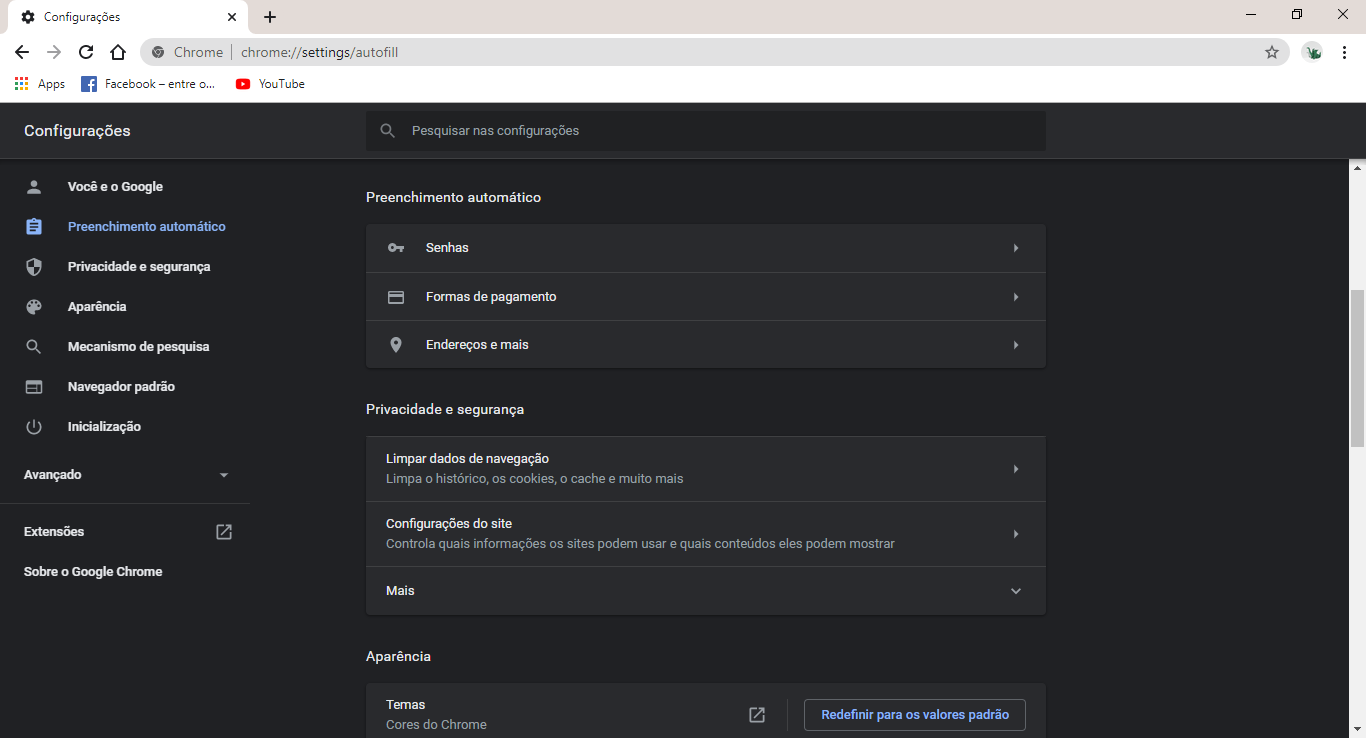
\includegraphics[width=0.8\linewidth]{Figuras/Ch03/fig8.9}
\end{frame}


\begin{frame}{Navegadores}
	\begin{block}{Alternativas}
		\begin{itemize}
			\item O Google Chrome \textbf{não é o único} navegador com essas funções, e há outros como o Opera, que também conta com uma \textbf{barra lateral} de acesso a algumas \textbf{redes sociais}, e o Mozilla Firefox que possui um \textbf{mini player} de vídeos.
		\end{itemize}
	\end{block}
	
	\bigskip
	
	\begin{minipage}{0.49\linewidth}
		\centering
		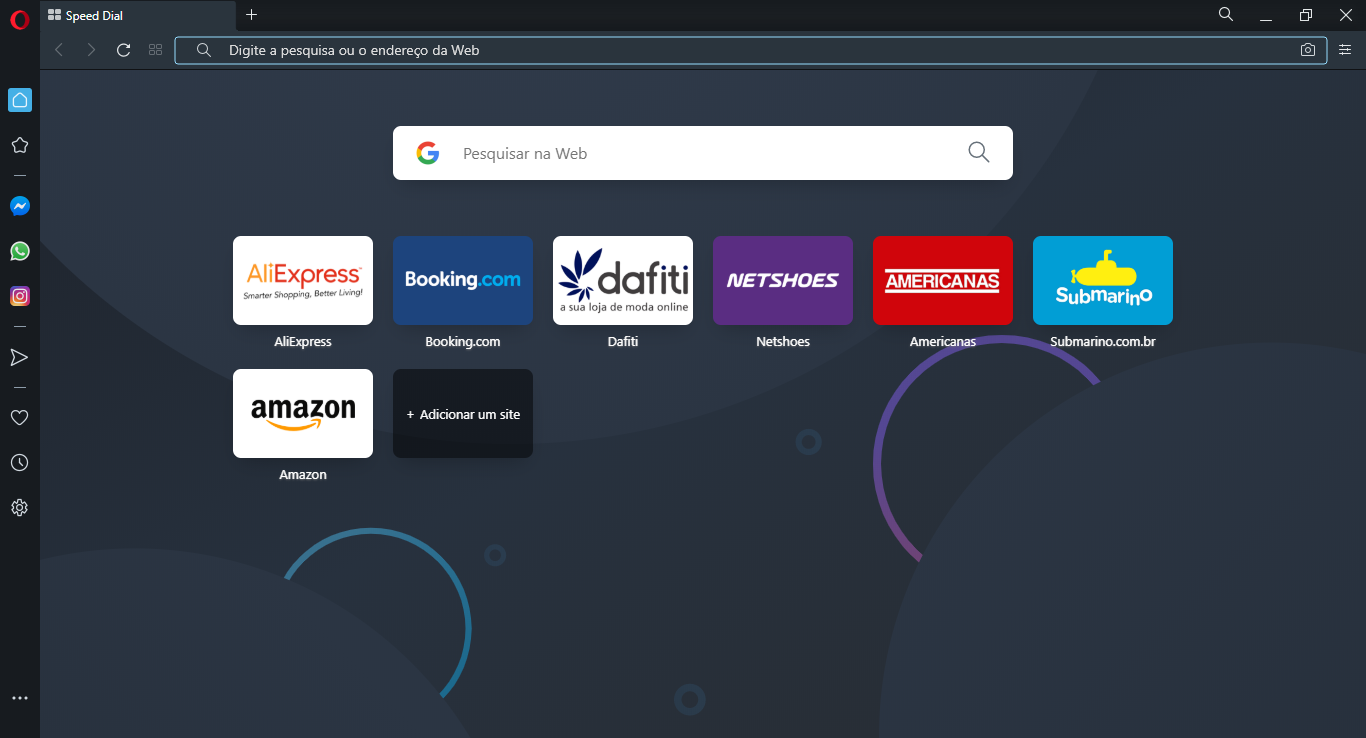
\includegraphics[width=1\linewidth]{Figuras/Ch03/fig8.4}
	\end{minipage}\hfill
	\begin{minipage}{0.49\linewidth}
		\centering
		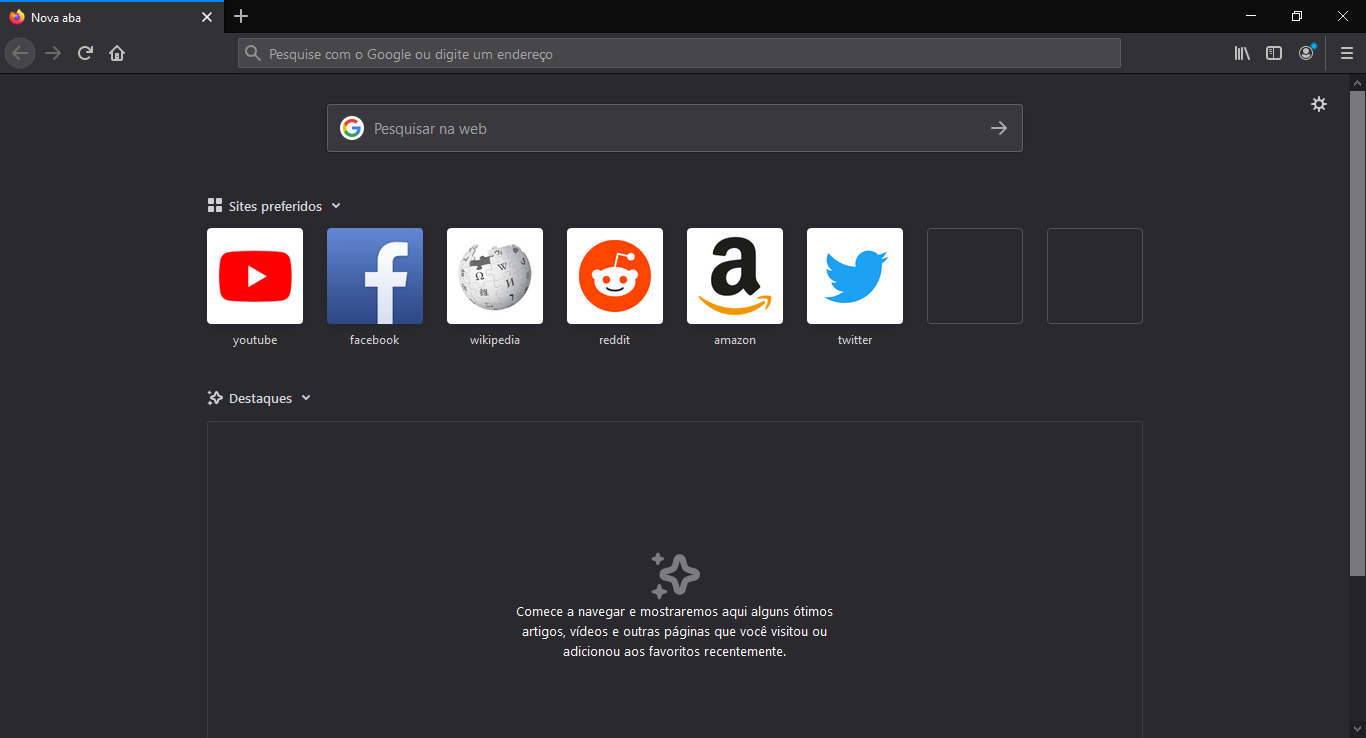
\includegraphics[width=1\linewidth]{Figuras/Ch03/fig8.5}
	\end{minipage}
\end{frame}


\begin{frame}{Navegadores}
	\begin{block}{Alternativas}
		\begin{itemize}
			\item O navegador padrão do Windows foi, por muitos anos, o \textit{Internet Explorer}, que tem fama por ser \textbf{lento} e \textbf{difícil de usar}.
			\item Hoje em dia, a Microsoft (empresa que produz o Windows) já lançou uma \textbf{alternativa}, que é o \textit{Microsoft Edge}.
		\end{itemize}
	\end{block}
	
	\bigskip
	
	\begin{minipage}{0.49\linewidth}
		\centering
		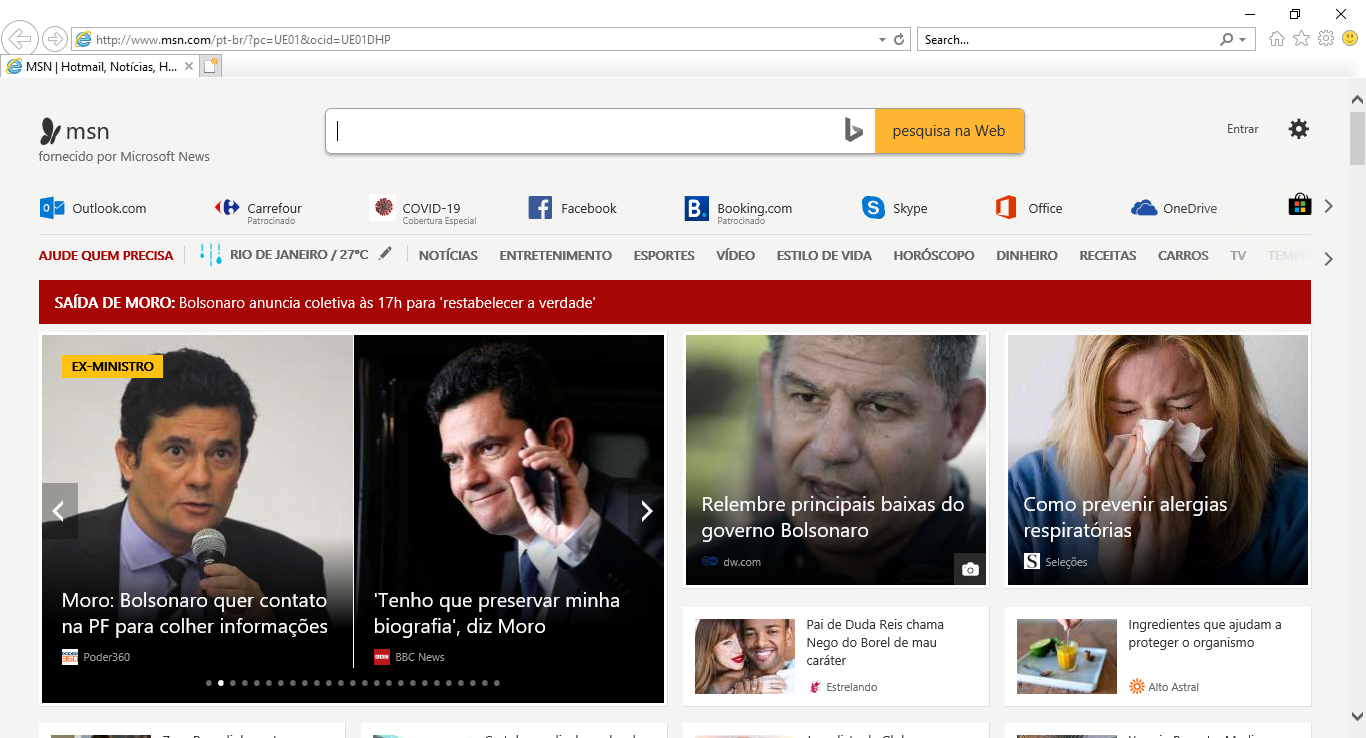
\includegraphics[width=1\linewidth]{Figuras/Ch03/fig8.1}
	\end{minipage}\hfill
	\begin{minipage}{0.49\linewidth}
		\centering
		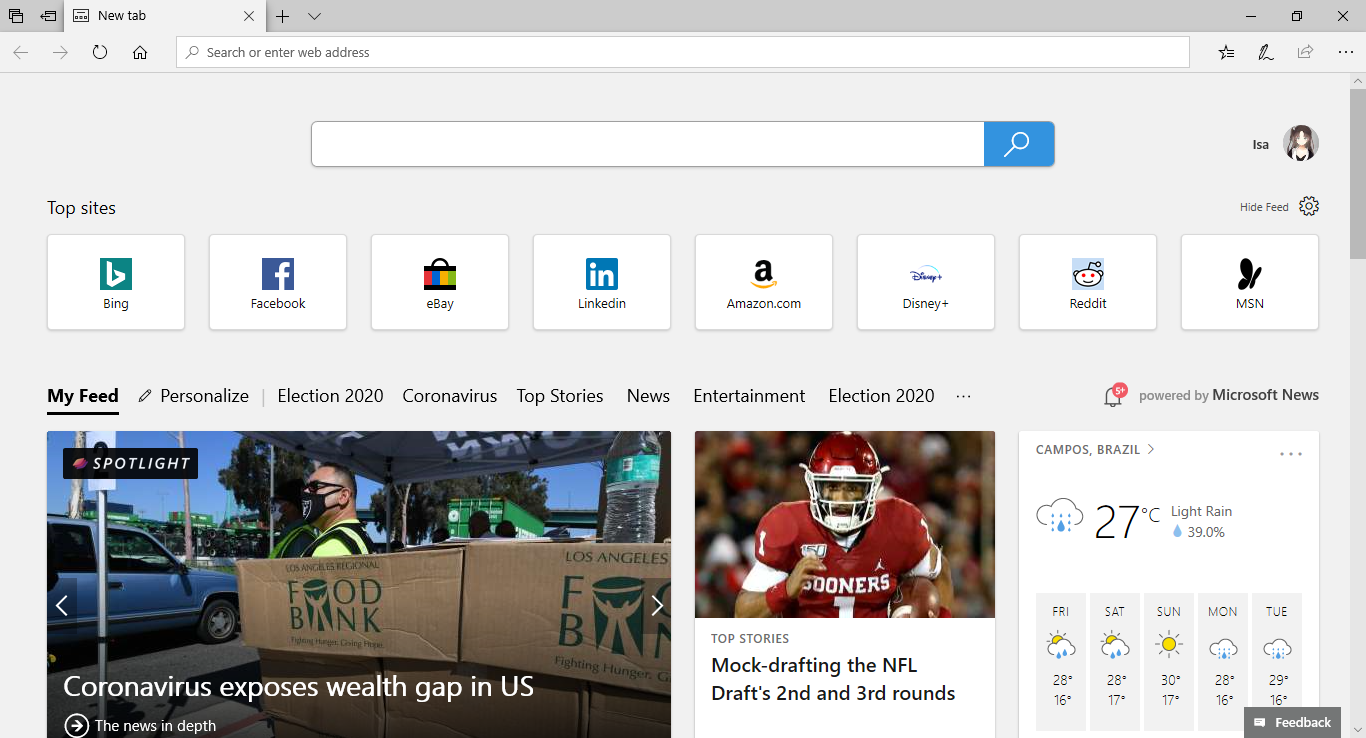
\includegraphics[width=1\linewidth]{Figuras/Ch03/fig8.3}
	\end{minipage}
\end{frame}


\begin{frame}{Navegadores}
	\begin{block}{Extensões}
		\begin{itemize}
			\item Vários navegadores também contam com expansibilidade de funcionalidade através de \textbf{extensões}.
			\item É possível usar uma extensão para ver a \textbf{cotação do dólar}, \textbf{marcar o tempo de uso} da internet ou até \textbf{bloquear anúncios}.
		\end{itemize}
	\end{block}

	\centering
	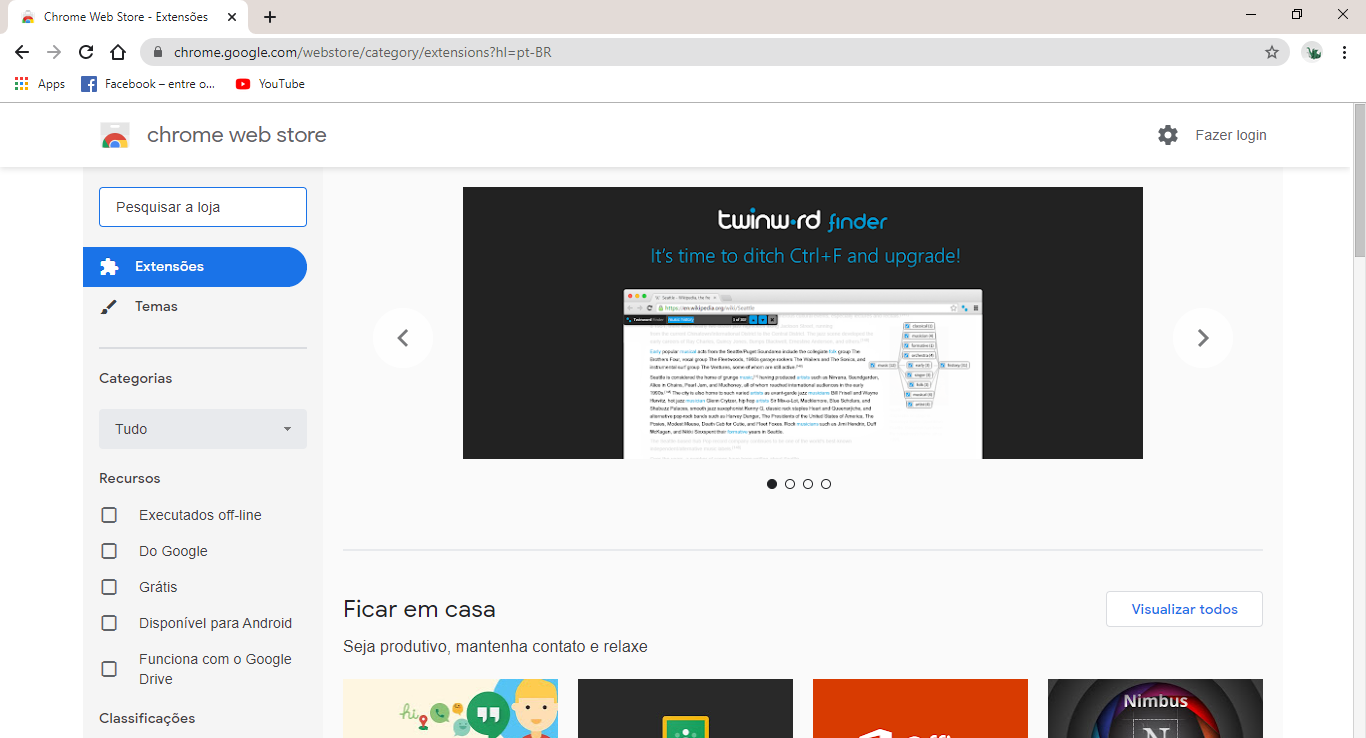
\includegraphics[width=0.7\linewidth]{Figuras/Ch03/fig8.13}
\end{frame}


\begin{frame}{Navegadores}
	\begin{block}{Privacidade}
		\begin{itemize}
			\item Eles pegam o conteúdo desejado, e \textbf{exibem} de uma forma agradável.
			\item Esse conteúdo, porém, pode ser acessado de \textbf{várias} maneiras: diretamente, indiretamente, com encriptação, etc.
			\item Normalmente, os navegadores acessam todo o conteúdo desejado de \textbf{forma direta}, e isso faz com que estejamos expostos a todo tipo de vigilância: um site pode facilmente \textbf{rastrear seu IP}, ou \textbf{coletar informações sobre você}.
		\end{itemize}
	\end{block}
	
	%	\centering
	%	\includegraphics[width=0.7\linewidth]{Figuras/Ch03/fig}
\end{frame}


\begin{frame}{Navegadores}
	\begin{block}{TOR}
		\begin{itemize}
			\item Uma ferramenta como o \textbf{TOR} é necessária para que possamos navegar sem essas preocupações, pois ela acessa a rede de \textbf{forma indireta}.
			\item Isso também nos permite acessar os \textbf{sites escondidos}, pois estes \textbf{não} estão disponíveis através de DNS (não tem um ``nome'' que podemos digitar para chegar neles).
			\item Não que seja algo recomendável acessar esses sites, pelo contrário, a maioria está escondida pois lida com \textbf{conteúdo ilegal}, ou porque possui \textbf{dados pessoais} de outras pessoas, que podem estar encriptados.
			\item Mas o que é \textbf{encriptação}?
		\end{itemize}
	\end{block}

	%	\centering
	%	\includegraphics[width=0.7\linewidth]{Figuras/Ch03/fig}
\end{frame}


\begin{frame}{Internet}
	\begin{block}{Encriptação}
		\begin{itemize}
			\item Encriptação é o \textbf{conjunto de técnicas utilizadas para ``esconder'' dados}.
			\item Digamos que você deseja enviar uma \textbf{mensagem secreta} para alguém, uma possibilidade é vocês \textbf{combinarem um código} como o do exemplo abaixo:
		\end{itemize}
	\end{block}

	\medskip

	\centering
	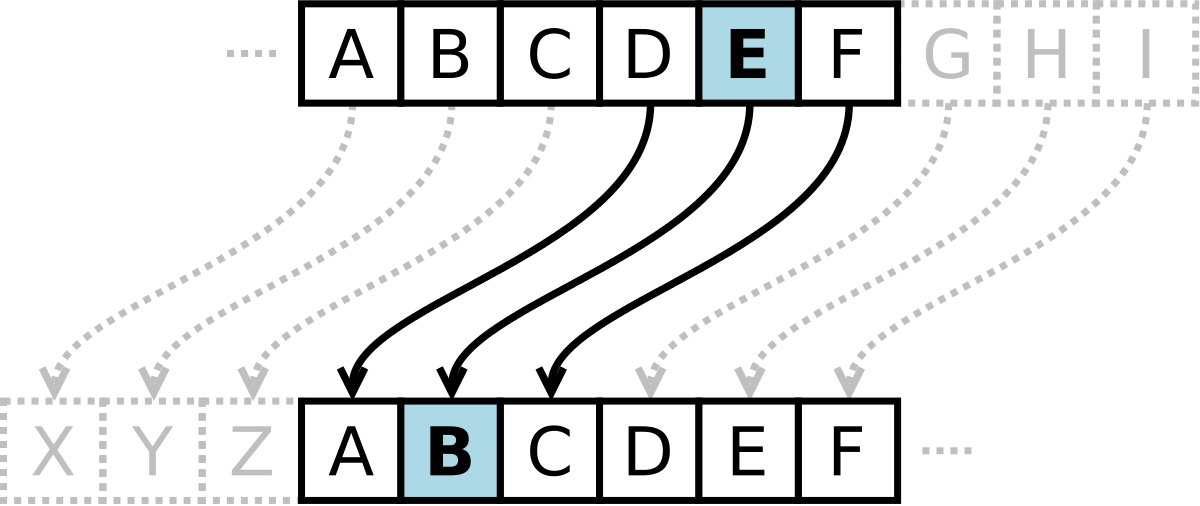
\includegraphics[width=0.7\linewidth]{Figuras/Ch03/fig11}
\end{frame}


\begin{frame}{Internet}
	\begin{block}{Encriptação}
		\begin{itemize}
			\item No exemplo, todas as letras são ``movidas'' 3 casas para a esquerda.
			\item Então, a frase ``Oi, tudo bom?'' vira ``Lf, qral ylj?''.
			\item Repare que a pontuação \textbf{não mudou}, e alguém poderia facilmente \textbf{adivinhar} a mensagem enviada.
			\item Se omitirmos a pontuação, podemos gerar textos bem \textbf{complexos}:
		\end{itemize}
	\end{block}

	\textsmaller[3]{l afpzl xjxobil firjfklrpb alfp alp xrqljósbfp ax cobkqb xzbiboxoxj xkqbp nrb l pfkxi sbojbiel xmxobzbppb kx mxppxabfox ab mbõbp prodfr l abpbkel al eljbj sboab x dbkqb nrb bpmboxsx zljbçlr x xqoxsbppxo x orx mfpxkal xp cxfuxp yoxkzxp mfkqxaxp kx zxmx kbdox al xpcxiql kãl eá kxax nrb jbklp pb mxobçx zlj rjx wbyox mloéj xppfj ieb zexjxj lp xrqljlyfifpqxp fjmxzfbkqbp zlj l mé kl mbaxi ax bjyoxfxdbj jxkqfkexj bj qbkpãl lp zxoolp xsxkçxkal obzrxkal zljl zxsxilp kboslplp nrb pbkqfppbj sfo kl xo x zefyxqx lp mbõbp gá xzxyxoxj ab mxppxo jxp l pfkxi ab zxjfkel ifsob mxox lp zxoolp sxf qxoaxo xfkax xidrkp pbdrkalp eá nrbj prpqbkqb nrb bpqx abjlox xmxobkqbjbkqb qãl fkpfdkfcfzxkqb pb x jriqfmifzxojlp mbilp jfiexobp ab pbjáclolp bufpqbkqbp kx zfaxab b mbixp jraxkçxp przbppfsxp axp qoêp zlobp ab zxax rj é rjx axp zxrpxp jxfp zlkpfaboásbfp alp bkdlodfqxjbkqlp ax zfozrixçãl xrqljósbi lr bkdxooxcxjbkqlp pb nrfpbojlp rpxo l qbojl zloobkqb}
\end{frame}


\begin{frame}{Internet}
	\begin{block}{Encriptação}
		\begin{itemize}
			\item Esse texto criptografado é o primeiro parágrafo da obra ``Um ensaio sobre a cegueira'', que rendeu um \textbf{prêmio Nobel} de literatura à José Saramago, seu autor.
			\item O método que utilizamos é a ``cifra de César'', e é bem antigo, datando da época de Júlio César, político Romano, que usava essa cifra movida em 3 unidades (A$ \to $D) para criptografar \textbf{mensagens militares}.
			\item Com uma mensagem grande o suficiente e bom senso, \textbf{qualquer um} consegue \textbf{descriptografar} uma mensagem dessa cifra: ela é fraca.
			\item Por isso adotamos criptografias \textbf{mais complexas} para os meios virtuais, tão complexas que nem os computadores \textbf{mais poderosos do mundo} conseguiriam quebrar em \textbf{milhares de anos}.
			\item As ideias por trás disso são bastante \textbf{complexas}, e consistem em \textbf{algoritmos matemáticos} baseados em \textbf{problemas de divisibilidade}.
		\end{itemize}
	\end{block}
\end{frame}


%\begin{frame}{Internet}
%	\begin{block}{}
%		\begin{itemize}
%			\item Esse texto criptografado é o primeiro parágrafo da obra ``Um ensaio sobre a cegueira'', que rendeu um prêmio Nobel de literatura à José Saramago, seu autor.
%			\item A cifra de César é bem antiga, e data da época de Júlio César, político Romano, que usava essa cifra movida em 3 unidades (A$ \to $D) para criptografar mensagens militares.
%			\item Com uma mensagem grande o suficiente e bom senso, qualquer um consegue descriptografar uma mensagem dessa cifra: ela é fraca.
%			\item Por isso adotamos criptografias mais complexas para os meios virtuais, tão complexas que nem os computadores mais poderosos do mundo conseguiriam quebrar em milhares de anos.
%			\item As ideias por trás disso são bastante complexas, e consistem em algoritmos matemáticos baseados em problemas de divisibilidade. 
%		\end{itemize}
%	\end{block}
%\end{frame}


\section*{Exercícios}
\frame{
	\frametitle{Exercícios}
	\begin{block}{}
		01. O que você faria se pudesse acessar qualquer arquivo da internet? Você gostaria que outra pessoa pudesse ver tudo o que você faz no computador?
		
		\medskip
		
		02. Você já usou alguma das ferramentas que foram citadas? Qual sua maior dificuldade na hora de fazer um trabalho?
	\end{block}
}

\section*{Referências}

\frame{
	\frametitle{Referências e Exercícios Complementares}
	\begin{itemize}
		\item Gammack, John G.; Hobbs, Valerie; Pigott, Diarmuid (2011). The Book of Informatics (em inglês) revisada ed. [S.l.]: Cengage Learning.
	\end{itemize}
	%\centering{\alert{Página 36 - \textbf{1.6.1 até 1.6.5, 1.6.17 até 1.6.19}}} \\
	%	\centering{\alert{Lista de exercícios 01}}
}